\documentclass{sigplanconf}

\usepackage{lgrind}
\usepackage[dvips]{graphicx}
\usepackage{verbatim}
\pagestyle{plain}

%% This bit allows you to either specify only the files which you wish to
%% process, or `all' to process all files which you \include.
%% Krishna Sethuraman (1990).

\typein [\files]{Enter file names to process, (chap1,chap2 ...), or `all' to
process all files:}
\def\all{all}
\ifx\files\all \typeout{Including all files.} \else \typeout{Including only \files.} \includeonly{\files} \fi

\begin{document}

% -*-latex-*-
% $Log: not supported by cvs2svn $
% Revision 1.1  2008/08/25 17:36:14  thies
% *** empty log message ***
%
% Revision 1.7  2001/02/08 18:53:16  boojum
% changed some \newpages to \cleardoublepages
%
% Revision 1.6  1999/10/21 14:49:31  boojum
% changed comment referring to documentstyle
%
% Revision 1.5  1999/10/21 14:39:04  boojum
% *** empty log message ***
%
% Revision 1.4  1997/04/18  17:54:10  othomas
% added page numbers on abstract and cover, and made 1 abstract
% page the default rather than 2.  (anne hunter tells me this
% is the new institute standard.)
%
% Revision 1.4  1997/04/18  17:54:10  othomas
% added page numbers on abstract and cover, and made 1 abstract
% page the default rather than 2.  (anne hunter tells me this
% is the new institute standard.)
%
% Revision 1.3  93/05/17  17:06:29  starflt
% Added acknowledgements section (suggested by tompalka)
%
% Revision 1.2  92/04/22  13:13:13  epeisach
% Fixes for 1991 course 6 requirements
% Phrase "and to grant others the right to do so" has been added to
% permission clause
% Second copy of abstract is not counted as separate pages so numbering works
% out
%
% Revision 1.1  92/04/22  13:08:20  epeisach
\title{Language and Compiler Support for Stream Programs}

\author{William Thies}
\department{Department of Electrical Engineering and Computer Science}
% If the thesis is for two degrees simultaneously, list them both
% separated by \and like this:
% \degree{Doctor of Philosophy \and Master of Science}
%\degree{Doctor of Philosophy of Science in Computer Science and Engineering}
\degree{Doctor of Philosophy}
\degreemonth{December} \degreeyear{2008} \thesisdate{\today}

\prevdegrees{~ \\ 
Bachelor of Science, Computer Science and Engineering\\
Massachusetts Institute of Technology, 2001 \\
~ \\
Bachelor of Science, Mathematics\\
Massachusetts Institute of Technology, 2002 \\
~ \\
Master of Engineering, Computer Science and Engineering \\
Massachusetts Institute of Technology, 2002 \\
~ \\
}

%% By default, the thesis will be copyrighted to MIT.  If you need to copyright
%% the thesis to yourself, just specify the `vi' documentclass option.  If for
%% some reason you want to exactly specify the copyright notice text, you can
%% use the \copyrightnoticetext command.
%\copyrightnoticetext{\copyright IBM, 1990.  Do not open till Xmas.}

% If there is more than one supervisor, use the \supervisor command
% once for each.
\supervisor{Saman Amarasinghe}{Associate Professor}

% These are optional, and enabled with reader.sty
%\reader{Arvind}{Professor}
%\reader{Srini Devadas}{Professor}

% This is the department committee chairman, not the thesis committee
% chairman.  You should replace this with your Department's Committee
% Chairman.
\chairman{Terry P. Orlando}{Chair, Department Committee on Graduate Students}

% Make the titlepage based on the above information.  If you need
% something special and can't use the standard form, you can specify
% the exact text of the titlepage yourself.  Put it in a titlepage
% environment and leave blank lines where you want vertical space.
% The spaces will be adjusted to fill the entire page.  The dotted
% lines for the signatures are made with the \signature command.
\maketitle

% The abstractpage environment sets up everything on the page except
% the text itself.  The title and other header material are put at the
% top of the page, and the supervisors are listed at the bottom.  A
% new page is begun both before and after.  Of course, an abstract may
% be more than one page itself.  If you need more control over the
% format of the page, you can use the abstract environment, which puts
% the word "Abstract" at the beginning and single spaces its text.

%% You can either \input (*not* \include) your abstract file, or you can put
%% the text of the abstract directly between the \begin{abstractpage} and
%% \end{abstractpage} commands.

% First copy: start a new page, and save the page number.
\cleardoublepage
% Uncomment the next line if you do NOT want a page number on your
% abstract and acknowledgments pages.
% \pagestyle{empty}
\setcounter{savepage}{\thepage}
\begin{abstractpage}
Due to the high data rates involved in audio, video, and signal
processing applications, it is imperative to compress the data to
decrease the amount of storage used.  Unfortunately, this implies that
any program operating on the data needs to be wrapped by a
decompression and re-compression stage.  Re-compression can incur
significant computational overhead, while decompression swamps the
application with the original volume of data.

In this paper, we present a program transformation that greatly
accelerates the processing of compressible data.  Given a program that
operates on uncompressed data, we output an equivalent program that
operates directly on the compressed format.  Our transformation
applies to stream programs, a restricted but useful class of
applications with regular communication and computation patterns.  Our
formulation is based on LZ77, a lossless compression algorithm
utilized by ZIP, and immediately applies to simpler formats such as
Apple Animation, Microsoft RLE, and Targa.

We implemented a simple subset of our techniques in the StreamIt
compiler, which emits executable plugins for two popular video editing
tools: MEncoder and Blender.  For common operations such as color
adjustment and video compositing, computing directly on compressed
data offers a speedup roughly proportional to the overall compression
ratio.  For our benchmark suite of 12 videos in Apple Animation
format, speedups range from 1.1x to 471x, with a median of 15x.

\end{abstractpage}

% Additional copy: start a new page, and reset the page number.  This way,
% the second copy of the abstract is not counted as separate pages.
% Uncomment the next 6 lines if you need two copies of the abstract
% page.
% \setcounter{page}{\thesavepage}
% \begin{abstractpage}
% Due to the high data rates involved in audio, video, and signal
processing applications, it is imperative to compress the data to
decrease the amount of storage used.  Unfortunately, this implies that
any program operating on the data needs to be wrapped by a
decompression and re-compression stage.  Re-compression can incur
significant computational overhead, while decompression swamps the
application with the original volume of data.

In this paper, we present a program transformation that greatly
accelerates the processing of compressible data.  Given a program that
operates on uncompressed data, we output an equivalent program that
operates directly on the compressed format.  Our transformation
applies to stream programs, a restricted but useful class of
applications with regular communication and computation patterns.  Our
formulation is based on LZ77, a lossless compression algorithm
utilized by ZIP, and immediately applies to simpler formats such as
Apple Animation, Microsoft RLE, and Targa.

We implemented a simple subset of our techniques in the StreamIt
compiler, which emits executable plugins for two popular video editing
tools: MEncoder and Blender.  For common operations such as color
adjustment and video compositing, computing directly on compressed
data offers a speedup roughly proportional to the overall compression
ratio.  For our benchmark suite of 12 videos in Apple Animation
format, speedups range from 1.1x to 471x, with a median of 15x.

% \end{abstractpage}

\cleardoublepage

\newpage
~ \vspace{-3.7\baselineskip}\\
\enlargethispage{0.3\baselineskip}
\section*{Acknowledgments}

I would like to start by expressing my deepest gratitude to my
advisor, colleague and friend, Saman Amarasinghe.
%Saman's committment to me has been downright scary.
%Simply put, Saman has changed my life.
%Simply put, Saman has been the mentor of a lifetime.
From 4am phone calls in Boston to weeks of one-on-one time in Sri
Lanka and India, Saman invested {\it unfathomable} time and energy
into my development as a researcher and as a person.  His extreme
creativity, energy, and optimism (not to mention mad PowerPoint
skills!) have been a constant source of inspiration, and whenever I am
at my best, it is usually because I am asking myself: {\it What would
Saman do}?  Saman offered unprecedented freedom for me to pursue
diverse interests in graduate school -- including weeks at a time
working with other groups -- and served as a fierce champion on my
behalf in every possible way.  I will forever treasure our deep sense
of shared purpose and can only aspire to impact others as much as he
has impacted me.

%Like a Papa Bear, any arguments between the two of us would be 
%completely dwarfed by the fierce battles he would wage on my behalf.

\vspace{-8pt}\paragraph*{Contributors to this dissertation} Many
people made direct contributions to the content of this dissertation.
The StreamIt project was a fundamentally collaborative undertaking,
involving the extended efforts of over 27 people.  I feel very lucky
to have been part of such an insightful, dedicated, and fun team.
Section~\ref{sec:streamit-project} provides a technical overview of
the entire project, including the division of labor.  In what follows
I am listing only a subset of each person's actual contributions.
Michael Gordon, my kindred Ph.D. student throughout the entire
StreamIt project, led the development of the parallelization
algorithms (summarized in Chapter~4), the Raw backend and countless
other aspects of the compiler.  Rodric Rabbah championed the project
in many capacities, including contributions to cache optimizations
(summarized in Chapter~4), teleport messaging (Chapter~3), the MPEG2
benchmarks, an Eclipse interface, and the Cell backend.  Michal
Karczmarek was instrumental in the original language design (Chapter
2) and teleport messaging, and also implemented the StreamIt scheduler
and runtime library.  David Maze, Jasper Lin, and Allyn Dimock made
sweeping contributions to the compiler infrastructure; I will forever
admire their skills and tenacity in making everything work.

Central to the StreamIt project is an exceptional array of
M.Eng. students, who I feel very privileged to have interacted with
over the years.  Andrew Lamb, Sitij Agrawal, and Janis Sermulins led
the respective development of linear optimizations, linear statespace
optimizations, and cache optimizations (all summarized in Chapter~4).
Janis also implemented the cluster backend, with support for teleport
messaging (providing results for Chapter~3).  Matthew Drake
implemented the MPEG2 codec in StreamIt, while Jiawen Chen implemented
a flexible graphics pipeline and Basier Aziz implemented mosaic
imaging.  Daviz Zhang developed a lightweight streaming layer for the
Cell processor; Kimberly Kuo developed an Eclipse user interface for
StreamIt; Juan Reyes developed a graphical editor for stream graphs;
and Jeremy Wong modeled the scalability of stream programs.  Kunal
Agrawal investigated bit-level optimizations in StreamIt.  Ceryen Tan
is improving StreamIt's multicore backend.

The StreamIt project also benefited from an outstanding set of
undergraduate researchers, who taught me many things.  Ali Meli, Chris
Leger, Satish Ramaswamy, Matt Brown, and Shirley Fung made important
contributions to the StreamIt benchmark suite (detailed in Chapter~2).
Steve Hall integrated compressed-domain transformations into the
StreamIt compiler (providing results for Chapter~5).  Qiuyuan Li
worked on a StreamIt backends for Cell, while Phil Sung targeted a
GPU.

%Qiuyuan Li worked on a StreamIt backend for the Cell processor, while
%Phil Sung worked on a backend for graphics processors.

Individuals from other research groups also impacted the StreamIt
project.  Members of the Raw group offered incredible support for our
experiments, including Anant Agarwal, Michael Taylor, Walter Lee,
Jason Miller, Ian Bratt, Jonathan Eastep, David Wentzlaff, Ben
Greenwald, Hank Hoffmann, Paul Johnson, Jason Kim, Jim Psota, Nathan
Schnidman, and Matthew Frank.
%
\newpage
\enlargethispage{0.3\baselineskip}
%
~ \vspace{-1.3\baselineskip}\\
\noindent Hank Hoffmann, Nathan Schnidman, and Stephanie Seneff also
provided valuable expertise on designing and parallelizing signal
processing applications.  External contributors to the StreamIt
benchmark suite include Ola Johnsson, Mani Narayanan, Magnus
Stenemo, Jinwoo Suh, Zain ul-Abdin, and Amy Williams.  Fabrice
Rastello offered key insights for improving our cache optimizations.
Weng-Fai Wong offered guidance on several projects during his visit
to the group.  StreamIt also benefited immensely from regular and
insightful conversations with stakeholders from industry, including
Peter Mattson, Richard Lethin, John Chapin, Vanu Bose, and Andy Ong.

Outside of the StreamIt project, additional individuals made direct
contributions to this dissertation.  In developing our tool for
extracting stream parallelism (Chapter~6), I am indebted to Vikram
Chandrasekhar for months of tenacious hacking and to Stephen McCamant
for help with Valgrind.  I thank Jason Ansel, Chen Ding, Ronny
Krashinsky, Viktor Kuncak, and Alex Salcianu, who provided valuable
feedback on manuscripts that were incorporated into this dissertation.
I am also grateful to Arvind and Srini Devadas for serving on my
committee on very short notice, and to Marek Olszewski for serving as
my remote agent of thesis submission!

\vspace{-8pt}\paragraph*{The rest of the story} Throughout my life,
I have been extremely fortunate to have had an amazing set of
mentors who invested a lot of themselves in my personal growth.  I
thank Thomas ``Doc'' Arnold for taking an interest in a nerdy high
school kid, and for setting him loose with chemistry equipment in a
Norwegian glacier valley -- a tactic which cemented my interest in
science, especially the kind you can do while remaining dry.
%a tactic which ignited not only my interest in science, but also in
%girls.
I thank Scott Camazine for taking a chance on a high school programmer
in my first taste of academic research, an enriching experience which
%was not only enriching and fun, but also 
opened up many doors for me in the future.  I thank Vanessa Colella
and Mitchel Resnick for making my first UROP experience a very
special one, as evidenced by my subsequent addiction to the UROP
program.  I thank Andrew Begel for teaching me many things, not
least of which is by demonstration of his staggering commitment,
capacity, and all-around coolness in mentoring undergraduates.  I'm
especially grateful to Brian Silverman, a mentor and valued friend
whose unique perspectives on everything from Life in StarLogo to
life on Mars have impacted me more than he might know.  I thank
Markus Zahn for excellent advice and guidance, both as my
undergraduate advisor and UROP supervisor.  Finally, I'm very
grateful to Kath Knobe, who provided unparalleled mentorship during
my summers at Compaq and stimulated my first interest in compilers
research.

Graduate school brought a new set of mentors.  I learned a great
deal from authoring papers or proposals with Anant Agarwal, Srini
Devadas, Fredo Durand, Michael Ernst, Todd Thorsen, and
Fr\'{e}d\'{e}ric Vivien, each of whom exemplifies the role of a
faculty member in nurturing student talent.  I am also very grateful
to Srini Devadas, Martin Rinard, Michael Ernst, and Arvind for being
especially accessible as counselors, showing interest in my work and
well-being even in spite of very busy schedules.  I could not have
imagined a more supportive environment for graduate study.

I thank Charles Leiserson and Piotr Indyk for teaching me about
teaching itself.  I will always remember riding the T with Charles
when a car full of Red Sox fans asked him what he does for a living.
Imagining the impressive spectrum of possible replies, I should not
have been surprised when Charles said simply, ``I teach''.  Nothing
could be more true, and I feel very privileged to have been a TA in
his class.

I'd like to thank my collaborators on projects other than StreamIt,
for enabling fulfilling and fun pursuits outside 
% the work described in 
of this dissertation.  In the microfluidics lab, I thank
J.P. Urbanski for many late nights ``chilling at the lab'', his
euphemism for a recurring process whereby he manufactures chips and
I destroy them.  His knowledge, determination, and overall good
nature are truly inspiring.  I also learned a great deal from David
Craig, Mats Cooper, Todd Thorsen, and Jeremy Gunawardena, 
%
\newpage
\enlargethispage{0.5\baselineskip}
%
~ \vspace{-1.5\baselineskip}\\
\noindent who were extremely supportive of our foray into
microfluidics.  I thank Nada Amin for her insights, skills, and
drive in developing our CAD tool, and for being an absolute pleasure
to work with.

%In the microfluidics lab, I learned an immense amount from
%J.P. Urbanski, microfluidic wizard extraordinaire whose work ethic
%is as intense as it is understated -- never again will I think
%lightly of a late night ``chilling at the lab''.

I'm very thankful to my collaborators in applying technology towards
problems in socio-economic development, from whom I've drawn much
support.  First and foremost is Manish Bhardwaj, whose rare
combination of brilliance, determination, and selflessness has been
a deep inspiration to me.  I also thank Emma Brunskill, who has been
a tremendous collaborator on many fronts, as well as
%whose independence and resourcefulness are always humbling.  
%I'm very grateful to Emma Brunskill, Somani Patnaik, 
Sara Cinnamon, Goutam Reddy, Somani Patnaik and Pallavi Kaushik for
being incredibly talented, dedicated, and fun teammates.
%I thank the Venerable Tenzin Priyadarshi and Scott Kennedy for
%valuable support and guidance.
%
%Further in the past, 
I am very grateful to Libby Levison for involving me in my first
project at the intersection of technology and development, without
which I might have gone down a very different path.  I also thank
Samidh Chakrabarti for being a great officemate and friend, and my
first peer with whom I could investigate this space together.

I am indebted to the many students and staff who worked with me on
the TEK project, including Marjorie Cheng, Tazeen Mahtab, Genevieve
Cuevas, Damon Berry, Saad Shakhshir, Janelle Prevost, Hongfei Tian,
Mark Halsey, and Libby Levison.  I also thank Pratik Kotkar,
Jonathan Birnbaum, and Matt Aasted for their work on the Audio Wiki.
I would not have been able to accomplish nearly as much without the
%continuous 
insights, dedication, and hard work of all these individuals.

% leaving out sri lanka guys, since it's not released:
% - Thayaparan Kailainathan
% - Mahendrakumar Senthivel
% - Thayarupan Rajendram
%
% leaving out some TEK authors who I don't even know:
% - Alexandro Artola
% - Binh D. Vo
% - Yuliya Litvak
% - Sheldon Chan
% - Sid Henderson

Graduate school would be nothing if not for paper deadlines, and I
feel very lucky to have been down in the trenches with such bright,
dependable, and entertaining co-authors.  Of people not already cited
as such, I thank Marten van Dijk, Blaise Gassend, Andrew Lee, Charles
W. O'Donnell, Kari Pulli, Christopher Rhodes, Jeffrey Sheldon, David
Wentzlaff, Amy Williams, and Matthias Zwicker for some of the best
end-to-end research experiences I could imagine.

Many people made the office a very special place to be.  Mary McDavitt
is an amazing force for good, serving as my rock and foundation
throughout many administrative hurricanes; I can't thank her enough
for all of her help, advice, and good cheer over the years.  I'm also
very grateful to Shireen Yadollahpour, Cornelia Colyer, and Jennifer
Tucker, whose helpfulness I will never forget.  Special thanks to
Michael Vezza, system administrator extraordinaire, for his extreme
patience and helpfulness in tending to my every question, and fixing
everything that I broke.

I thank all the talented members of the Commit group, and especially
the Ph.D. students and staff -- Jason Ansel, Derek Bruening, Vikram
Chandrasekhar, Gleb Chuvpilo, Allyn Dimock, Michael Gordon, David
Maze, Michal Karczmarek, Sam Larsen, Marek Olszewski, Diego Puppin,
Rodric Rabbah, Mark Stephenson, Jean Yang, and Qin Zhao.  On top of
tolerating {\it way} more than their fair share of StreamIt talks,
they offered the best meeting, eating, and traveling company ever.  I
especially thank Michael Gordon, my officemate and trusted friend, for
making 32-G890 one of my favorite places -- I'm really going to miss
our conversations (and productive silences!)

I'd like to extend special thanks to those who supported me in my job
search last spring.  I feel very grateful for the thoughtful counsel
of dozens of people on the interview trail, and especially to a few
individuals (you know who you are) who spent many hours talking to me
and advocating on my behalf.  This meant a great deal to me.  I also
thank Kentaro Toyama and others at MSR India for being very flexible
with my start date, as the submission of this thesis was gradually
postponed!

I am extremely fortunate to have had a wonderful support network to
sustain me throughout graduate school.  To the handful of close
friends who joined me for food, walks around town, or kept in touch
from a distance: thank you for seeing me through the thick and thin.
I'd like to especially call out to David Wentzlaff, Kunal Agrawal,
Michael Gordon and Cat Biddle, who held front-row season tickets to my
little world and made it so much better by virtue of being there.

Finally, I would like to thank my amazingly loving and supportive
parents, who have always been 100\% behind me no matter where I am
in life.  I dedicate this thesis to them.

%% \clearpage
%% ~ \\ \vspace{1.1in} ~ \\
%% \begin{center}
%% {\bf \large Relation to Prior Publications}
%% \end{center}
\section*{Relation to Prior Publications}
This dissertation alternately extends and summarizes prior
publications by the author.  Chapters 1 and 2 are significantly more
detailed than prior descriptions of the StreamIt
language~\cite{thies-cc02,thies-can02,amarasinghe-ijpp05} and include
an in-depth study of the StreamIt benchmark suite that has yet to be
published elsewhere.  Chapter~3 subsumes the prior description of
teleport messaging~\cite{thies-ppopp05}, including key changes to the
semantics and the first uniprocessor scheduling algorithm.  Chapter~4
is a condensed summary of prior
publications~\cite{gordon-asplos02,lamb-pldi03,agrawal-cases05,sermulins-lctes05,gordon-asplos06},
though with new text that often improves the exposition.  Chapter~5
subsumes the prior report on compressed-domain
processing~\cite{thies07compression}, offering enhanced functionality,
performance, and readability.  Chapter~6 is very similar to a recent
publication~\cite{thies-micro07}.  Some aspects of the author's work
on StreamIt are not discussed in this
dissertation~\cite{karczmarek-lctes03,chen-graphics05}.

Independent publications by other members of the StreamIt group are
not covered in this
dissertation~\cite{kuo05,drake-ipdps06,zhang_lightweight_2007}.  In
particular, the case study of implementing MPEG2 in StreamIt provides
a nice example-driven exposition of the entire
language~\cite{drake-ipdps06}.

%\vspace{1in}
%\begin{center}
%{\bf \large Funding Acknowledgment}
%\end{center}
\section*{Funding Acknowledgment}
This work was funded in part by the National Science Foundation
(grants EIA-0071841, CNS-0305453, ACI-0325297), DARPA (grants
F29601-01-2-0166, F29601-03-2-0065), the DARPA HPCS program, the MIT
Oxygen Alliance, the Gigascale Systems Research Center, Nokia, and a
Siebel Scholarship.
\clearpage

% NOT ACKNOWLEDGING:
%
% - Meha Senthil?
%
% StreamIt:
% - Vijay Saraswat
% - Ryan Newton
% - Ken Steele provided an IPAQ for some of the experiments in Chapter~4.
%
% Teaching:
% - David Liben Nowell
% 
% Microfluidics:
% - natalie andrew
%
% IIH:
% - Seema Kacker
% - Sourav Dey
% - Ajit Dash
% - Alex Krull
% - Oliver Venn
% - Jessica Leon
% - Nikhil Nadkarni
% - Catherine Dunn
%
% All these details:
%
% I am indebted to many additional students and collaborators who
% helped to pursue goals at the intersection of technology and
% development in my graduate school career.
%
% For external contributions to TEK, from Elsevier I thank Ammy
% Votglander, Craig Scott, Jeremy Alder, Spencer de Groot, and
% Christian Pruvost; from First Mile Solutions, I thank Rich
% Fletcher, Amir Alexander Hasson, and Olufemi Omojola; from the
% People's First Network, I thank David Leeming.  
%
% At Innovators In Health, I thank Manish Bhardwaj, Sara Cinnamon,
% Goutam Reddy, Emma Brunskill, Somani Patnaik, Pallavi Kaushik,
% Seema Kacker, Sourav Dey, Ajit Dash, Alex Krull, Oliver Venn,
% Jessica Leon, Nikhil Nadkarni, and Catherine Dunn.  
%
% I also thank Rich Fletcher, Michael Gordon, Jonathan Jackson,
% Jhonatan Rotenberg, Luis Sarmenta, Ammy Votglander for many
% conversations benefiting this research.  I would not have been
% able to accomplish nearly as much without the steadfast
% dedication and help of all of these individuals.


%%%%%%%%%%%%%%%%%%%%%%%%%%%%%%%%%%%%%%%%%%%%%%%%%%%%%%%%%%%%%%%%%%%%%%
% -*-latex-*-

\pagestyle{plain}
%  % -*- Mode:TeX -*-
%% This file simply contains the commands that actually generate the table of
%% contents and lists of figures and tables.  You can omit any or all of
%% these files by simply taking out the appropriate command.  For more
%% information on these files, see appendix C.3.3 of the LaTeX manual. 
\tableofcontents
\newpage
\listoffigures
\newpage
\listoftables


\section{Introduction}


Stream computing represents an increasingly important class of
applications. In streaming codes, there is an abundance of parallelism that
is easier to extract compared to traditional desktop workloads (e.g.,
pointer-based computing). As a result, the extraction of parallelism
in streaming codes does not require heroic efforts, and thus,
processors can deliver higher performance with significantly lower
power costs. This is especially important since
leading microprocessor companies have realized that modern general
purpose architectures are near their  performance limits for  the
amount of power they consume. Thus, the future will place a greater
emphasis on exploiting the properties of streaming workloads in
conventional von~Neumann architectures.

Streaming is a model of computation that uses sequences of data
and computation kernels to expose concurrency and locality for
efficiency~\cite{wss}. In general purpose processors, improving locality 
translates to an effective management of the memory hierarchy at all
levels, including the register file. In this paper, we present a
methodology for compiling streaming codes to general purpose,
cache-based architectures. We first introduce a simple model for
reasoning effectively about the caching behavior of streaming
workloads. This model serves as a foundation for several {\it cache-aware
optimizations} that are geared toward the concomitant increase of instruction
and data {\it temporal locality}. These
optimization lead to significantly better utilization of the memory
system, and as such, they deliver performance gains ranging from 11
to 99\% for our streaming benchmark suite.

The context for our work is StreamIt, an architecture-independent
language that is engineered for streaming
applications~\cite{streamitcc}. It adopts the 
Cyclo-Static Dataflow~\cite{BELP96} model of computation which is a
generalization of Synchronous Dataflow~\cite{LM87-i} (SDF).  
SDF is a popular  model that  is well suited for
streaming codes. In SDF, computation is represented as a graph
consisting of {\it  actors} connected by communication channels; the
actors consume  and produce a constant number  of items from their
input and output  channels every time they execute. SDF is appealing
because it is amenable to static scheduling and optimization. 

From a general purpose architecture's point of view, actors represent
computation kernels, and the communication between actors represents
data buffers that must be streamed to and from the processor. Thus
the size of an actor and the
order of actor executions are critical properties that
impact the performance of the instruction cache. For example, the
compiler must make sure the actor's code size is not
greater than the instruction cache. Furthermore, we must {\it scale}
the execution of the actor so that it runs several times before we move
on to some other actor in the stream 
graph. This serves to $(i)$ amortize the cost of fetching the actor's
instructions into the cache from memory (an expensive operation), $(ii)$
improve the instruction temporal locality, and $(iii)$ improve overall
performance. However, as our cache model will show, we 
cannot arbitrarily scale the execution frequency of an actor. This
is because actors produce data that must be buffered, and therefore,
we must also consider the amount of data an actor produces and
consumes if we are to adequately manage the data cache. This paper is unique
in that it is the first to present a unified optimization methodology
that simultaneously considers instruction and data locality for
mapping streaming computation to cache-based architectures.

In terms of improving the data cache behavior, the compiler schedules
actor firing such that the producer-consumer locality is
preserved. Furthermore,  the compiler may {\it fuse}
together two or more actors to form a coarser grained kernel.
The fusion allows for better register allocation as we can
destroy the arrays used to buffer data between the actors and replace
the corresponding array references with scalars.  It also allows for
various competing implementations for managing the buffers between the
fused actors.  This paper evaluates several implementation
alternatives (for buffer management) and evaluates their performance.

The methodology for fusing actors leverages a distinguishing StreamIt
characteristic, namely, the hierarchical organization of
the stream graph. Furthermore, the algorithm for fusing actors applies
for the various topologies allowed by StreamIt.
It also considers another distinguishing characteristics of StreamIt,
namely the {\tt peek} operation whereby an actor may inspect data
items in its input buffer without consuming them until some future
execution. While peeking is a powerful language feature, it does pose
some challenges to the compiler and the cache optimizations. Peeking
also impacts the choice for the best buffer management strategy, as our
study will show.

%% the comment about p3 and itanium not being embedded architectures
%% is out of the blue! need a better transition.
Cache-aware fusion alone delivers significant performance gains, although our
evaluation shows that fusion with scaling leads to the best
performance on a general purpose, cache-based architecture. For our
experiments, we use two different processors: a superscalar out-of-order
processor, and an in-order VLIW processor. The former is a Pentium~3
whereas the latter is an Itanium~2. While these architectures are not
particularly suited for an embedded system, they do exhibit some
properties that are worthy of investigation. Furthermore, that we can
demonstrate measurable performance gains on real systems is far more
convincing than using a simulation-based environment. We chose the
Pentium~3 processor because it has very few registers in its
instruction set architecture. The Itanium by contrast has a much 
larger and richer repertoire of registers. The two architectures serve
to validate our cache-aware optimizations, in that we expect an
architecture with more register to benefit more from optimization such
as scalar replacement. On average, fusion leads to a 47\% improvement
on the Pentium~3, and 50\% on the Itanium~2.

The two architectures also differ in terms of their memory system
organization. The Itanium is an in-order VLIW processor and does not
tolerate a memory stall as well as its out-of-order
counterpart. Therefore we expect different gains from the scaling
optimization which amortize the long access latencies for instruction
and data caches. On average, scaling leads to a 21\% improvement on
the Itanium~2, and 17\% on the Pentium~3.

While both scaling and fusion lead to modest performance gains, we
must combine the two to deliver the best possible performance. When we
do so, we can further improve the performance of our benchmarks by
53\% on average for the Pentium~3, and 55\% for the Itanium~2.

\subsection{Summary of Contributions}

This paper makes the following contributions:
\begin{itemize}

\item A cache model for stream computing that provides a quantitative
estimate of the caching performance for any sequence of actor
executions.

\item A cache-aware scheduling heuristic that judiciously increases
the multiplicity of actors, improving instruction and data locality
while not exceeding the data cache.

\item A cache-aware partitioning policy that judiciously fuses
adjacent actors into a single component, enabling local optimizations
while not exceeding the instruction cache.

\item An optimized buffer management policy, termed ``copy-shift with
execution scaling'', which out-performs a traditional rotating buffer
in a detailed micro-benchmark analysis.

\item A fully automatic implementation of the above techniques in the
StreamIt compiler.

\item An experimental evaluation across 11 streaming benchmarks,
demonstrating performance improvements of up to 99\%.
\end{itemize}

\subsection{Paper Roadmap}

The remainder of the paper is organized as follows. Section~\ref{sec:streamit}
describes StreamIt and introduces our motivating example.
Section~\ref{sec:cache-model} introduces our cache model for 
reasoning about the performance of a streaming
computation. Section~\ref{sec:cache-opt} describes our cache-aware
optimizations, and Section~\ref{sec:buffer} describes the 
optimization enabled by fusion. Section~\ref{sec:evaluation} describes
our evaluation methodology and present our experimental
analysis. Sections~\ref{sec:related-work}~and~\ref{sec:conclusion}
discuss related work and concludes the paper.

\section{Multicore Streaming Layer}\label{ch:lib}

Emerging multicore architectures provides an excellent target for
streaming language compilers for a number of reasons:
\begin{itemize}
\item Individual cores are optimized for computation, often supporting
short vector operations in the form of SIMD instructions.
\item Limited memory capacity on a core is not a severe
limitation for streaming actors. In a stream program, actors typically
embody computation, are independent of each other, have extremely
local data-access patterns, and generally have small code sizes.
\item The availability of high-bandwidth and low-latency on-chip
communication network enables a large number of scheduling options
which would not be feasible for other targets, such as computing
clusters.
\end{itemize}

In a multicore setting, a streaming language compiler (or programmer)
must address the following challenges:
\begin{enumerate}
\item Generating code that explicitly manages data communication
  (e.g., DMA operations). Architectures that provide an asynchronous
  communication model also require pipelining the data transfers (e.g.,
  double-buffering) to increase efficieny and throughput.
\item For architectures with a finite local store on a core, the code,
  input and output buffers, and the state required by the computation
  must be tightly packaged to fit into the local memory. This
  consideration is akin to locality enhancing optimizations for
  architectures with caches.
\item Performing high-level optimizations and scheduling to achieve a
  balanced distribution of work among the cores, avoiding excess
  communication, transforming code to improve efficiency, and
  ultimately delivering high processing throughput.
\end{enumerate}

The purpose of the multicore streaming layer (MSL) is to abstract
\textsf{(1)} and provide facilities that simplify \textsf{(2)} and
\textsf{(3)}. The MSL frees a compiler or programmer from needing to
deal with the details of the architecture communication model,
allowing it to focus on exploring high-level optimization and
scheduling choices. The main goal of the MSL is to provide a generic
framework for controlling and dispatching computation to multicores
that simplifies scheduling operations. The low level details that are
specific to individual platforms are embedded in the MSL library
implementation, and hidden from the programmer or the compiler. As a
result, the MSL can provide a common platform for mapping streaming
computation to multicore and enhance portability.

\section{MSL Constructs}

There are are a number of stream-oriented languages drawing from
domains such as functional, dataflow, CSP and synchronous
programming~\cite{survey97}. The MSL assumes an architecture-independent
programming language for high-performance stream programming. It
requires that the stream program presented for execution simply
consists of a dataflow graph expressing the computation. Nodes in the
graphs embody computation (e.g., actors, filters, some encapsulated
code block), and edges indicate data dependencies between
input and output buffers attached to the compute nodes.

An execution of a stream program is an ordered sequence of node
firings. Each node follows a set of execution steps that consume a
number of items from each input channel and produce a number of items
onto each output channel.

There are two basic constructs in the MSL: \emph{filters} and
\emph{buffers}. A filter represents a generic actor that exposes a
work function which conceptually runs infinitely. Filters may be
stateful and can read from multiple input buffers and write to multiple
output buffers. While a filter can correspond directly to a
single filter in the program, a compiler can also perform
optimizations such as fusing multiple filters into a single
coarse grained MSL filter~\cite{asplos02}. Work functions are opaque to the MSL.

\emph{Buffers} are contiguous regions of data that are reserved for
temporarily storing input or output data. All buffers are circular,
and the MSL library maintains head and tail pointers for each buffer
that indicate where data begins and ends. Conceptually, a buffer has
front and back ends; data towards the front of a buffer originated
earlier in the execution of the program.

Conceptually, a filter consists of two major components, \emph{code}
and \emph{state}, as well as basic properties that describe its work
function such as the number of input and output buffers. \emph{Code} is
a single contiguous block of arbitrary data that may contain constant
data and instructions that define multiple functions; the MSL only
requires that it contain a function with a specific signature, which
is used as the work function. Code for a filter is intended to be a
single modular component that can be easily relocated to different
local store addresses on different cores. As such, it should not
reference any absolute addresses, such as in absolute branches or
loads, or modify itself.\footnote{If the user can accept limitations,
such as not being able to relocate filter code or tying code to a
single core, these restrictions can be ignored.} The latter constraint
means that code should not contain any global variables; instead, all
global variables should be declared and accessed through fields in the
filter's state. \emph{State} contains all mutable data that must be
maintained across iterations of the work function. State for different
filters is disjoint, and filter code cannot access mutable global
state. Although a filter's code and state must reside in core local
store when the filter's work function is running, every filter must
have a permanent store for them in memory. The MSL provides
facilities for loading code onto cores and copying state between local
store and memory.

Before a filter can be run on a core, it must be loaded onto the core
through the MSL library. The user provides the library with the
properties of the filter and the local store (LS) address of its work
function; the library initializes a control block that describes the
loaded filter in local store, the LS address of which identifies the
loaded filter in all future operations until it is unloaded. If the filter is stateful, the
library also copies its state into local store from its permanent
store in memory. Code for the filter must be separately copied into
local store through the library, but can be located anywhere as long
as the correct work function address is provided to the library. When
the user is done with a loaded filter, it can unload the filter
through the library, causing the library to copy the filter's state
back to its permanent store in memory. Stateful filters can be loaded
on at most one core at any time, while stateless filters can be
simultaneously loaded on any number of cores (hence facilitating
coarse-grained data parallelism).

This separation of code and state allows the user additional control
over how and when core local store is used. Since code is constant,
the user can preload the code of a filter onto a core even while the
filter is loaded on another core (and thus its state is owned by that
core) in preparation for loading it on the first core in the
future. If multiple (possibly stateful) filters have identical code,
only one copy of it needs to reside in memory or a core's local store
and it can be shared. When a filter is not being run, its code does
not need to be present in core local store, leaving more space free
for buffering (local store management is discussed in more detail
below).

The library provides similar facilities for allocating buffers on
cores. The size of a buffer must be a power of two, to allow
wrap-around computations to be done with a single bit-wise \textsf{AND}
instruction. Buffers are identified by the LS address that their data
region starts at in core local store; when allocating a buffer, the
library initializes a control block located immediately before the
data region that stores the buffer's head and tail pointers and
participates in data transfers. As an additional step required before
a loaded filter can be run, the user must specify which buffers the
filter refers to.

%% The library does not provide memory management for core local store;
%% when filter code, filter control blocks, and buffers are allocated,
%% the user must manually specify their LS addresses and ensure that the
%% regions used by different constructs do not overlap.\footnote{The
%% library handles all resulting communication, such as copying filter
%% code and state.} This does not create as many difficulties as may
%% appear, as any memory management algorithm that can be implemented
%% internally by the library can just as easily be duplicated by the user
%% on the PPE. Moreover, allowing the user to explicitly manage local
%% store allows it to implement far more complex algorithms as
%% desired. Additionally, in this scheme, buffers and space occupied by
%% filter code and filter control blocks for stateless filters never need
%% to be explicitly deallocated -- the user can simply reuse the local
%% store region for other constructs after it is certain that they are no
%% longer in use.

Theoretically, the number of filters loaded and buffers allocated on a
core is limited only by available local store.
%% However, there is
%% generally no useful purpose in keeping more than two filters and their
%% associated buffers on a core at any time.

%% \subsection{PPE Constructs}

%% The library does not define a filter construct for the PPE. However, because all memory is addressable by PPE code, the user can easily create similar behavior.

%% The library defines a PPE or memory buffer construct that is an extension of the core buffer. PPE buffers are not required to be circular, and buffers that are non-circular have no size limitations. PPE buffers are identified by the address of their control block, and multiple buffers can refer to the same data region, with different head and tail pointers. This is used to implement certain StreamIt features with minimal overhead, such as duplicate splitters and data-parallel execution. Because of the limited size of core local store, this functionality was considered unnecessary for core buffers.

Conceptually, data produced during the execution of a program is
contained in exactly one buffer (which may be a core or PPE buffer)
until it is consumed. The MSL library provides facilities for moving
data between buffers on different processors.
 
\section{MSL Operations}

The MSL defines a simple set of operations to ease the mapping of stream
programs to multicores. A scheduler dispatches work items to cores by
issuing MSL commands, and is notified when cores complete
them. Each MSL command encapsulates a specific action to be
performed, and has parameters that are specified by the user. The
set of operations is divided into three main types:
\begin{itemize}
\item Filter commands: commands to load or unload filters, copy filter code into local store, attach filters to buffers, and run filters.
\item Buffer commands: commands to allocate buffers.
\item Data transfer commands: commands to move data between buffers in the local stores of different cores, or local store and memory.
\end{itemize}

As an example, the \textsf{filter\_run} command, which runs a loaded
filter, takes two parameters: the LS address of a loaded filter's
control block and the number of iterations for which to run the work function.
The user is responsible for ensuring that there is sufficient
data in input buffers and sufficient space in output buffers for all
specified iterations. Other commands have similar requirements. For a
complete description of all commands, see \cite{dxzhang-meng-07}.

The amount of work specified by a single command varies depending on
parameters to the command. Typically, work functions are small and thus \textsf{filter\_run} commands do
not take more than a few hundred microseconds to complete; some other
commands, such as allocating and attaching buffers, are auxiliary commands and complete almost immediately. This
allows the user to quickly change scheduling decisions and avoids
tying a core into any specific long-term action.

When the user issues a command to a core, it assigns the command an ID
that must be unique among all commands previously issued to that core
that have not completed. This ID is used to notify the user when the
core finishes executing the command.

\subsection{Dependencies}

In order to keep cores supplied with work at all times, it is
necessary to limit round-trips between the scheduler and the cores
during which the cores have no commands to execute. The MSL library
provides a general facility for queuing and ordering commands on
individual cores by allowing each command to specify a set of command
IDs on the core on which it depends. Commands issued to a core are
queued and executed only after all dependencies have finished.

At any time, a command that has been issued to a core can be either
\emph{queued} (a command with unfinished dependencies), \emph{active}
(a command with all dependencies satisfied and currently being
executed), or \emph{completed} (a command for which all work has been
done, but the user has not yet been notified). From the perspective of
the user, all commands that are active on a core are run
``concurrently''. When a command is issued, all dependency IDs that
have not been issued are considered to have already completed and are
ignored.

In effect, each core maintains a small dependency graph of commands
that represents a subset in time and space of the entire
schedule. The scheduler (which may be
user code, or a dynamic scheduler running on a control processor)
continually adds commands to the dependency graph, while the core
continually processes commands that have their dependencies
satisfied. To make full use of a core, it is only necessary for the
scheduler to ensure the dependency graph on the core is never
empty. The scheduler cannot remove commands once issued, but if it
keeps the dependency graph low-depth, it can quickly change the
pattern of work done by a core simply by issuing a different set of
new commands.

\subsection{Command Groups}

Each command has a small amount of data associated with it, consisting
of command-specific parameters in addition to generic ID and
dependency information. Typically, the user will be issuing sets of
related commands at once. To avoid the overhead of issuing each
command individually, the user can organize commands into groups; the
library only allows entire command groups to be issued.\footnote{To
issue a single command, the user can create a group containing only
that command.} Each group specifies a sequence of commands; until a
group is explicitly cleared, commands in the group are saved and can
be reissued in the future.

Since core local store is managed by the user, the user must provide
the library with an LS address where command data will be copied to
when it issues a command group. For dependency purposes, cores treat
commands in a group as having been issued in the order they appear in
the group. 

\subsection{Scheduler Interface}

Commands issued to different cores are completely independent; the
dependency graph on each core is strictly local. The scheduler serves
as the main point of synchronization between cores by adjusting the
commands it issues to a core in response to command completion
notifications from all cores.

The scheduler is mainly callback-driven. It registers a callback
function with the MSL library that is called whenever a command issued
to a core completes. The library maintains a per-core bitmap of
command IDs that have completed; the user can query this bitmap in the
callback to determine which commands have completed and respond
accordingly. Bits in the bitmap are set until explicitly acknowledged
by the user. After an ID has been acknowledged, it can be reused for
a new command issued to the core.

%% The library does not maintain a dependency graph on the PPE. Some core
%% commands have equivalents on the PPE provided as library functions,
%% which are run immediately when called.

%% Appendix~\ref{app:ui} contains complete specifications for the interface provided by the library to user code.

\subsection{Data Transfer}

Data transfer commands indirectly result in additional points of
synchronization between processors. A data transfer conceptually moves
data from the front of a source buffer to the back of a destination
buffer, and requires two commands: a command to transfer data out of
the source buffer, issued to the processor containing the source
buffer, and a command to transfer data into the destination buffer,
issued to the processor containing the destination buffer. Where
either buffer is located in memory, the user instead calls a library
function.

Splitting data transfers into a pair of commands with one on each
processor provides the user with explicit control over when the data
transfer occurs with respect to both processors. The library ensures
that the transfer does not occur until both commands become active on
their respective processors. The scheduler must ensure, via the
dependency graphs on cores or manually on a control processor, that
when a data transfer command becomes active on a processor, the local
buffer has sufficient data or space to fulfill the transfer.

%% Data transfers impose minor alignment requirements on the buffers
%% involved due to limitations of Cell's underlying DMA model.

There are no restrictions on the size of a data transfer (except for
the size of the buffers involved), but the same size must be specified
by both commands in the pair. Each data transfer command also
specifies the address and size of the opposing buffer, since this is
information the scheduler (or user) will know in advance; however,
buffer head and tail pointers, which are more difficult to track in
advance, are handled by the library. In addition, data transfer
commands have additional inter-core requirements that the user must
ensure are met across all cores.

This ``decoupling'' of data transfers simplifies the information the
scheduler needs to keep track of. When issuing commands to one core,
it usually does not need to be concerned with the state of other
cores; as long as pairs of data transfer commands are eventually
issued with the correct parameters and dependencies, the MSL library
will handle synchronization between buffers.

\subsection{Runtime Checks}

The MSL library implements a number of runtime checks that can be
enabled or disabled. When enabled, the library validates buffers
accesses to ensure that they contain sufficient data/space, and
performs additional checks to ensure that issued commands are
consistent. While this cannot identify all bugs in a schedule or
filter work function, it has nonetheless been very useful during the
development of the library, the dynamic scheduler, and test programs;
it has often exposed bugs that would otherwise only appear as a hung
program or incorrect output.


\section{Detailed Example}
\label{sec:example}

% dzm: this figure might just need to go.
\begin{figure*}
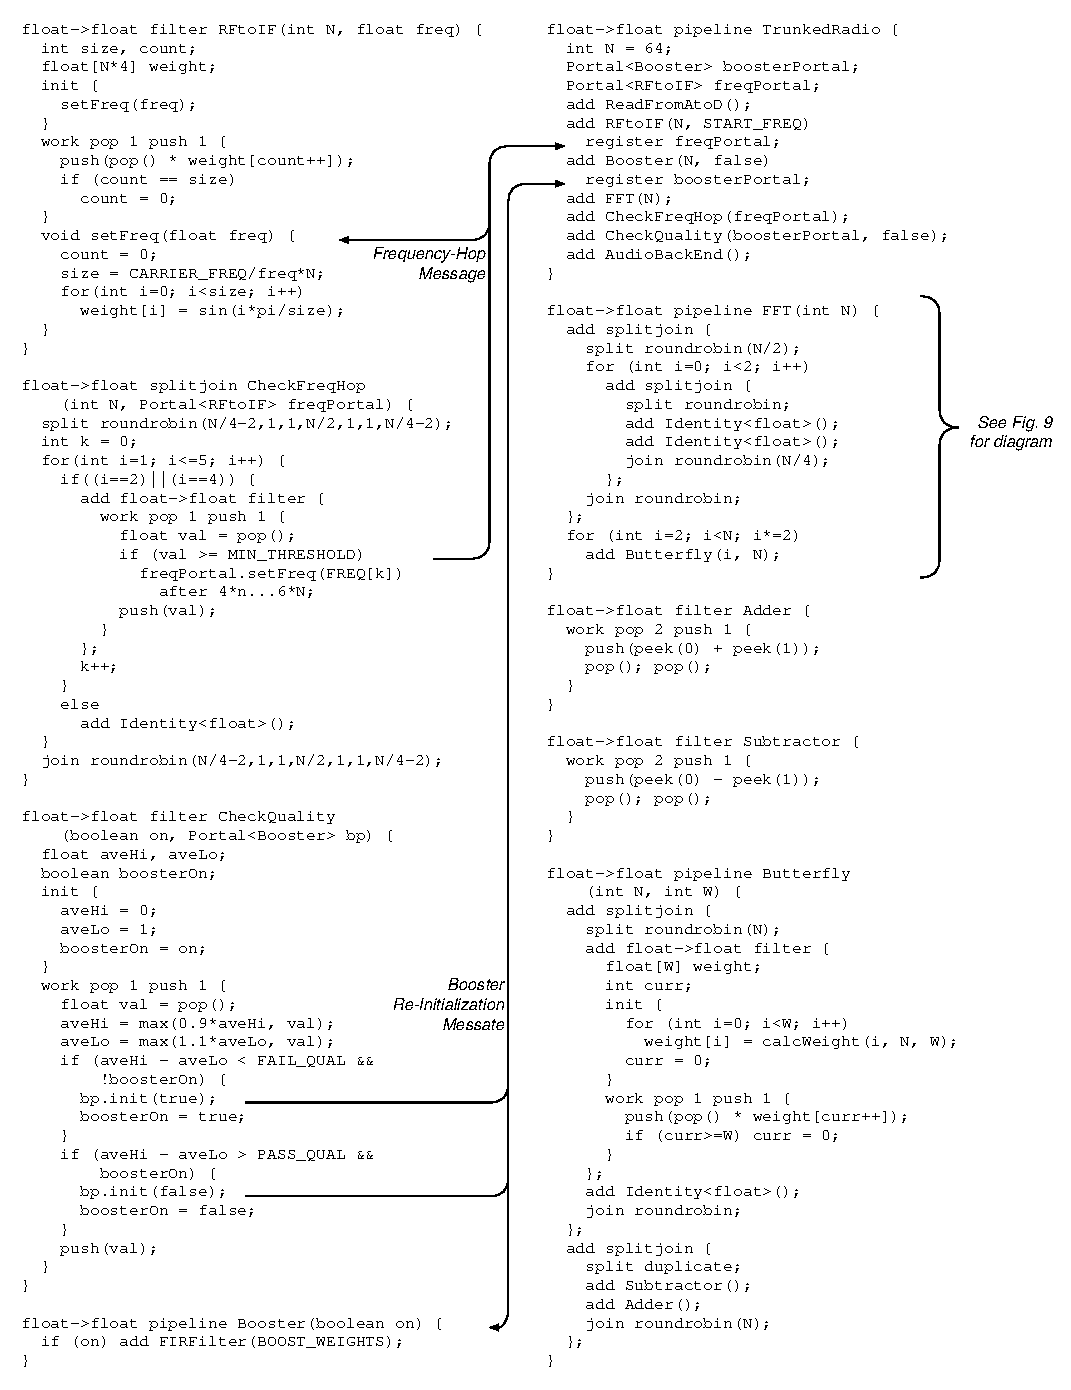
\includegraphics[width=\textwidth]{code-fm.eps}
\caption{StreamIt code for a software radio.  Arrows denote the paths
  of messages.}
\label{fig:radiocode}
\end{figure*}

We now discuss the StreamIt implementation of the Trunked Radio
illustrated in Fig.~\ref{fig:radiodiagram}.  The Trunked Radio is a
frequency-hopping system in which the receiver switches between a set of
known frequencies whenever it hears certain tones from the transmitter.

The toplevel class, \texttt{TrunkedRadio}, is implemented as a
seven-stage pipeline (see Fig.~\ref{fig:radiocode}).  The
\texttt{RFtoIF} stage modulates the input signal from RF to a
frequency band around the current IF frequency.  To support a change
in the IF frequency when frequency hopping occurs, the \texttt{RFtoIF}
filter contains a \texttt{setFreq} method that is invoked via a
message from the \texttt{CheckFreqHop} stage.  The message is sent
from \texttt{CheckFreqHop} with a latency range of $4N$ to $6N$, which
means that \texttt{RFtoIF} must deliver between $4N$ and $6N$ items
using the old modulation scheme before changing to the new frequency.

The optional \texttt{Booster} stage provides amplification for weak
signals, but is usually turned off to conserve power.  The
\texttt{Booster} is toggled by a re-initialization message from the
\texttt{CheckQuality} stage, which estimates the signal quality by the
shape of the frequency spectrum.  If all the frequencies have similar
amplitudes, \texttt{CheckQuality} assumes that the signal-to-noise
ratio is low and sends a message to activate the \texttt{Booster}.
This message is sent using best-effort delivery.

The \texttt{FFT} stage converts the signal from the time domain to the
frequency domain; please refer to p.~796 of \cite{clr} for a diagram
of the parallel FFT algorithm.  The StreamIt implementation consists
of a bit-reversal permutation followed by a series of
\texttt{Butterfly} stages.  The bit-reversal phase illustrates how
data can be reshuffled with just a few SplitJoin constructs (see
Fig.~\ref{fig:bitreverseorder}).  The \texttt{Butterfly}
stage--which is parameterized to allow for a compact representation of
the FFT--also employs split-joins to select groups of items for its
computation.  We believe that the StreamIt version of the FFT is clean
and intuitive, as the SplitJoin constructs expose the natural
parallelism of the algorithm.

%%% Local variables:
%%% TeX-master: "paper.tex"
%%% End:

%\section{Implementation and Evaluation}
\label{sec:results}

We have implemented a fully-functional prototype of the StreamIt
optimizing compiler as an extension to the Kopi Java Compiler, a
component of the open-source Kopi Project \cite{kopi}.  Our compiler
generates C code that is compiled with a StreamIt runtime library to
produce the final executable.  We have also developed a library in
Java that allows StreamIt code to be executed as pure Java, thereby
providing a verification mechanism for the output of the compiler.

The compilation process for streaming programs contains many novel
aspects because the basic unit of computation is a stream rather than
a procedure.  In order to compile stream modules separately, we have
developed a runtime interface--analogous to that of a procedure call
for traditional codes--that specifies how one can interact with a
black box of streaming computation.  The stream interface contains
separate phases for initialization and steady-state execution; in the
execution phase, the interface includes a contract for input items,
output items, and possible message production and consumption.  The
interface relies on the $min$ function to specify message timing in
terms of a stream's input tape.


We have evaluated our compiler with StreamIt versions of the following
applications: 1) A GSM Decoder, which takes GSM-encoded parameters as
inputs, and uses these to synthesize audible speech, 2) A system from
the Polymorphic Computing Architecture (PCA) \cite{pca} which
encapsulates the core functionality of modern radar, sonar, and
communications signal processors, 3) A software-based FM Radio with
equalizer, and 4) A performance test from the SpectrumWare system that
implements an Orthogonal Frequency Division Multiplexor (OFDM)
\cite{spectrumware}.  Table \ref{tab:benchmarks} gives characteristics
of the above applications including the number of filters implemented
and the size of the stream graph as coded.

\begin{table}[t]
\begin{center}
\scriptsize
\begin{tabular}{|l|r|r|r|} \hline
Benchmark & Lines & Filters & Graph Size\\
\hline \hline
PCA Demo & 484 & 5 & 7\\
\hline
FM Radio & 411 & 5 & 27\\
\hline
perftest4 & 347 & 5 & 20\\
\hline
GSM Decoder & 3050 & 11 & 21 \\
\hline
\end{tabular}
\vspace{-6pt}
\caption{\protect\small Application Characteristics}
\label{tab:benchmarks}
\vspace{-12pt}
\end{center}
\end{table}

%% \subsection{GSM Decoder}

%%   The decoder portion of the StreamIt GSM Vocoder takes GSM encoded
%% parameters as inputs, and uses these to synthesize audible speech.  This
%% is accomplished by processing the parameters through four main filters.
%% The RPE decoder filter produces some "pink noise" that very loosely
%% estimates the speech waveform, using quantized bit sequences and a
%% maximum value parameter from the encoded input.  This "pink noise" is
%% fed to the Long Term Prediction portion, which applies long-term
%% characteristics to the sequence through a delay filter within a feedback
%% loop.  The resulting signal is then sent to the Short Term Synthesis
%% filter, which decodes high frequency voice characteristics from the
%% encoded parameters and applies these to the signal.  Finally, the
%% Post-processing filter identifies peaks in the signal to make it audible.

%% \subsection{PCA Demo}

%% This application is representative of the core functionality needed by
%% modern radar, sonar, and communications signal processors.

In the Table~\ref{tab:performance}, we evaluate the performance of our
compiler by comparing the StreamIt implementation against either the
SpectrumWare implementation or (in the case of GSM) a hand-optimized C
version.  The StreamIt compiler is able to beat the SpectrumWare
performance by a factor of two for the PCA Demo and FM Radio.

For the GSM application, the extensively hand-optimized C version
incorporates many transformations that rely on the high-level
knowledge of the algorithm, and the StreamIt performs an order of
magnitude slower.

The StreamIt compiler infrastructure is far from complete. We are in
the process of discovering all the optimization possibilities in this
new domain.  We plan to implement many of the important optimizations.
Our code generation strategy currently has many inefficiencies. In the
future, we plan to generate optimized assembly code by interfacing
with a code generator.  We strongly believe that we can improve the
current performance by at least an order of magnitude on
uniprocessors. And we have yet to take advantage of the inherent data
and pipeline parallelism in StreamIt programs for parallel execution!

\begin{table}[t]
\begin{center}
\scriptsize
\begin{tabular}{|l|r|r|r|r|} \hline
& \multicolumn{2}{|c|}{StreamIt} &  \multicolumn{2}{|c|}{Hand Coded}\\
\hline 
Benchmark & Baseline & Fusion & Spectra & C \\
\hline \hline
PCA Demo & 1.3 & - & 3.4 & N/A\\
\hline
FM Radio & 5.8 & 4.9 & 9.9 & N/A\\
\hline
perftest4 & 330 & - & 330 & N/A\\
\hline
GSM Decoder & 4.88 & - & N/A & .47\\
\hline
\end{tabular}
\vspace{-6pt}
\caption{\protect\small Performance Results (in $\mu$sec/output)}
\label{tab:performance}
\vspace{-12pt}
\end{center}
\end{table}
%\section{Mapping StreamIt Patterns to the Runtime Library}\label{ch:use}

There are a number of common execution patterns that can be used to run a StreamIt program (see section~\ref{ch:bg:str:exec}). To illustrate how these patterns can be mapped to the runtime library for Cell, we will refer to the FFT StreamIt benchmark as a concrete example. This program performs a 256-element fast Fourier transform. The program's stream graph consists of a single pipeline of 15 filters. Every filter in the pipeline is stateless (and hence data-parallel) and does not peek. A single complete execution of the stream graph processes a single set of 256 input elements (512 floats), producing the same number of output elements.

%% \begin{figure}[!htb]
%% \begin{center}
%% 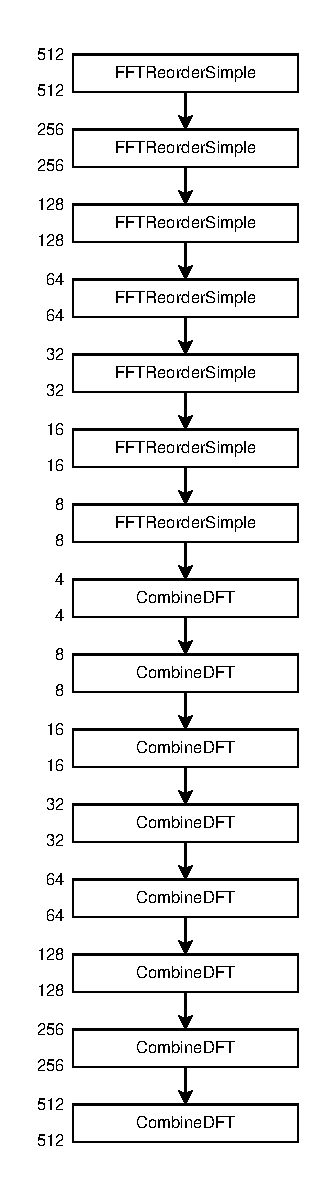
\includegraphics{figs/fftgraph}
%% \end{center}
%% \caption[Stream graph for 256-element FFT.]{Stream graph for 256-element FFT. A single execution of the stream graph pops and pushes 512 floats, since each element is a complex number whose components are interleaved on tapes.}
%% \label{fig:use:fftgraph}
%% \end{figure}

Data-parallel filters are the simplest to map to the library. The entire FFT pipeline can be fused into a single data-parallel filter that pops and pushes 512 floats per work function iteration. The fused filter can be data-parallelized over many SPEs: pseudocode to do this is illustrated in figure~\ref{fig:use:dp}. The \textsf{ext\_ppu\_spu\_ppu\_ex} library function starts an extended operation that loads the filter, allocates its buffers, and runs it for a large number of iterations.\footnote{The user still specifies all major parameters -- for example, the addresses to allocate buffers at and how many iterations each \textsf{filter\_run} command runs for.} The line containing \textsf{spulib\_poll\_while} synchronizes all SPEs; it returns only when all SPEs have finished and the callback has been run for each SPE.

\begin{figure}[!htb]
\begin{center}
\begin{tabular}{ll}
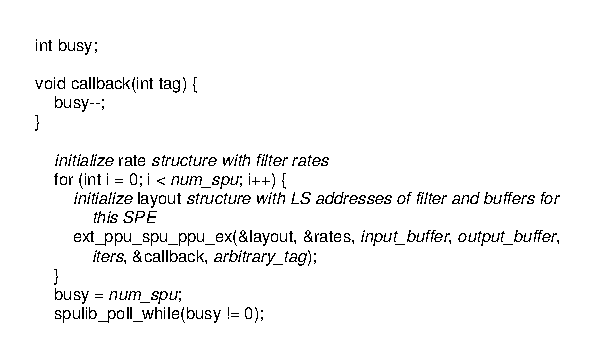
\includegraphics{figs/dpcode} & 
\includegraphics{figs/dp}
\end{tabular}
\end{center}
\caption[Pseudocode for running a data-parallel filter.]{Pseudocode for running a data-parallel filter. The figure on the right represents the state of each SPE as time passes. The horizontal line indicates synchronization by the PPE.}
\label{fig:use:dp}
\end{figure}

Course-grained software pipelining~\cite{asplos06} can be implemented similarly. Typically, the user will have assigned each filter in the steady state to an SPE and allocated and populated a buffer in memory for each channel. Pseudocode to execute a single iteration of the steady state is illustrated in figure~\ref{fig:use:swpipe}. Again, the line containing \textsf{spulib\_poll\_while} synchronizes all SPEs; this is necessary to ensure that sufficient input data has been produced for every filter in the next steady state iteration. For efficiency, the steady state should be sufficiently coarsened to amortize the overhead while SPEs are switching between filters and thus not performing any computation.

\begin{figure}[!htb]
\begin{center}
\begin{tabular}{ll}
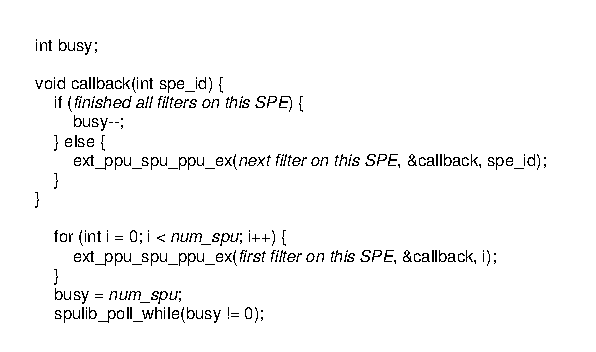
\includegraphics{figs/swpipecode} & 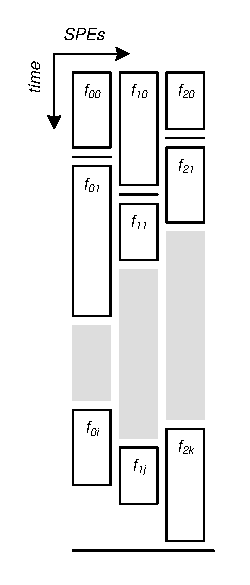
\includegraphics{figs/swpipe}
\end{tabular}
\end{center}
\caption[Pseudocode for running a course-grained software pipeline.]{Pseudocode for running a course-grained software pipeline. The figure on the right represents the state of each SPE as time passes. Horizontal lines indicate synchronization by the PPE.}
\label{fig:use:swpipe}
\end{figure}

Both patterns presented so far involve no direct SPE--SPE communication. An alternative implementation for FFT partially fuses the 15 filters in the StreamIt pipeline into a number of library filters, which are simultaneously run on different SPEs. These SPEs can transfer data between local stores directly, taking advantage of Cell's on-chip communication network and avoiding the extra latency to memory, as well as preventing memory from possibly becoming a bottleneck. Pseudocode to do this is illustrated in figure~\ref{fig:use:spepipecode}.

%% \begin{figure}[!htb]
%% \begin{center}
%% 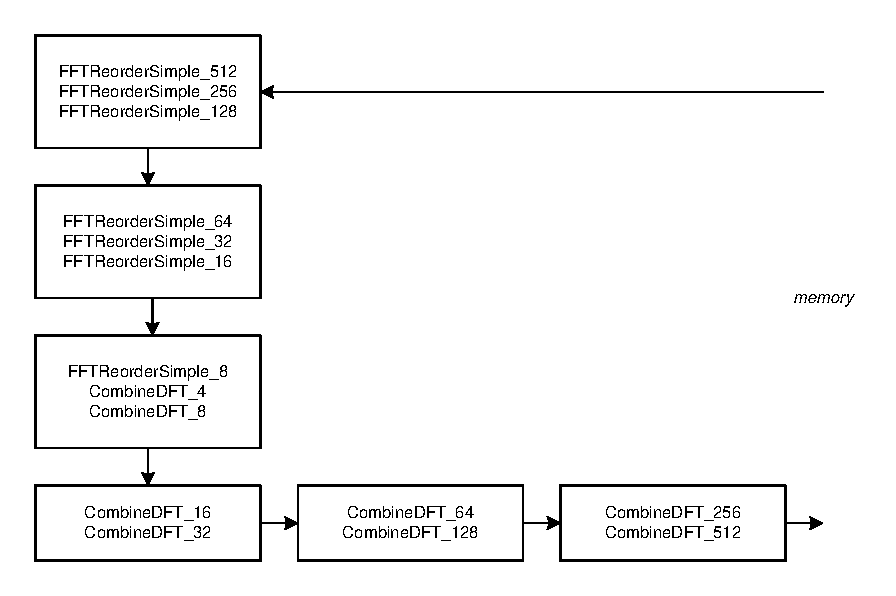
\includegraphics{figs/spepipe}
%% \end{center}
%% \caption{Pipelining FFT over six SPEs.}
%% \label{fig:use:spepipe}
%% \end{figure}

\begin{figure}[!htb]
\begin{center}
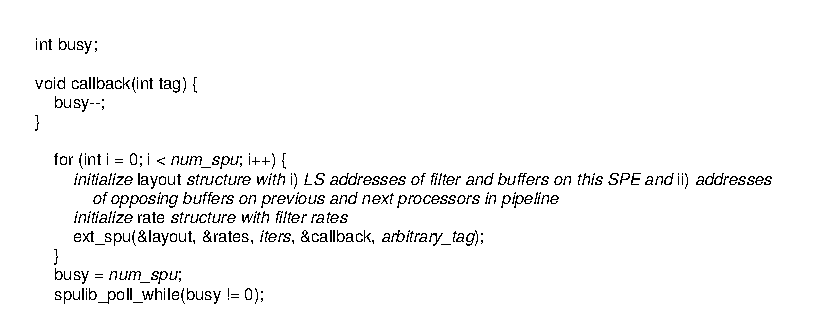
\includegraphics{figs/spepipecode}
\end{center}
\caption{Pseudocode for setting up an SPE--SPE pipeline.}
\label{fig:use:spepipecode}
\end{figure}

More complex scheduling choices require the user to provide more complex callback functions. For example, the communication overhead of loading a new filter onto an SPE can be hidden if the load is performed while the old filter is still running its last iterations.

The library allows the user to treat filters as individual schedulable entities, instead of having to consider complex lower-level operations. The pseudocode in figure~\ref{fig:use:dp} can be compared to the SPE code required to execute the same pattern (a single fused data-parallel filter) without using the library, illustrated in figure~\ref{fig:use:handcode}.

\begin{figure}[!htb]
\begin{center}
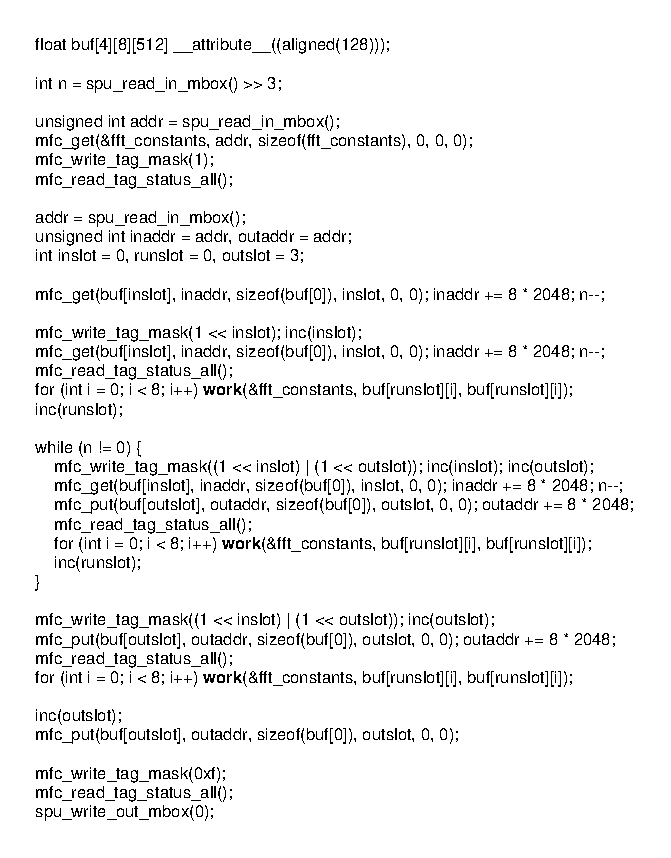
\includegraphics{figs/handcode}
\end{center}
\caption[SPE code for hand-coded implementation of data-parallel fused FFT.]{SPE code for hand-coded implementation of data-parallel fused FFT. The three bolded calls to \textsf{work} actually run the fused work function; the rest of the code performs double-buffered data transfers.}
\label{fig:use:handcode}
\end{figure}

This code is not overly complex, and will always be more efficient than using the library. However, this code is also specific to the filter and the execution pattern. The fused filter in FFT does not peek, and conveniently produces and consumes amounts of data that are compatible with Cell's DMA alignment requirements. The code would have to be significantly changed if a filter with slightly different rates were substituted. If multiple filters need to be run on an SPE, the code would then acquire additional logic to switch between filters. To run filters in an SPE--SPE pipeline, additional code would be needed to synchronize between SPEs. Using the library, the user does not need to deal with any of this.

\section{Splitters and Joiners}

In general, the type of fine-grained data reorganization performed by round-robin splitters and joiners cannot be directly implemented using Cell's DMA mechanism, which has strict alignment requirements. However, since the library supports filters with multiple input and/or output tapes, a compiler can simply define separate filters for each splitter and joiner. A compiler can also fuse a splitter or joiner with the upstream or downstream filter, respectively; the resulting filter has a much lower communication--computation ratio than an independent splitter or joiner.

The user can ignore duplicate splitters as long as the output of the upstream filter is buffered into memory. Because multiple PPE buffers can refer to the same data region, no duplication of data in memory is necessary. However, if the filters downstream of the splitter run on different SPEs, the same data must be copied to the local store of each SPE.

\section{Scheduling Stream Programs Using the MSL}\label{ch:ds}

Streaming programs typically allow for a lot of freedom in terms of
orchestrating the execution of the stream graph. This freedom is
afforded by the dataflow models of computation that many streaming
languages are founded on. In a stream program, the rules governing the
execution of a node or actor in the graph are often simple, and usually
reduce to having sufficient buffering on the input to an actor, and
sufficient buffering to store the output.

The execution of a stream program requires mapping and ordering actors
to cores, allocation of buffers, and managing data transfers between
buffers. Collectively, mapping, ordering, and buffer managements are
embodied in a schedule of execution.

It is possible to devise a schedule statically (e.g., compile time or
at graph creation time) or dynamically (e.g., runtime). The goal of a
scheduler is simply to maximize the throughput of the streaming
application. In the age of multicore architectures, a scheduler will
need to utilize the cores to increase concurrency and hence improve
the throughput of a given streaming application. 

A dynamic scheduler is conceptually easy to understand. The scheduler
maintains an internal representation of a given stream graph (e.g.,
list or priority queue). In a multicore architecture, when there is a
core available, the scheduler scans its internal representation of the
stream graph, and determines which actor is ready to fire.
The scheduler assigns the actor to the available core. The core is
also informed where the input buffer for the actor resides in memory,
and where in memory to commit (buffer) the output of the actor for its
successors. The scheduler then updates its internal representation to
indicate the actor firings and implement a fairness policy to assure
overall progress (e.g., a round-robin scheduler).

For stream graphs that are ``well-behaved'', dynamic scheduling
generally does not present any advantages over static
scheduling. Dynamic scheduling inevitably involves additional
communication and scheduling overhead due to extra filter loading and
unloading, buffer management, and scheduling computation. When all
filters in a program are data-parallel, a static scheduler can make
full use of all cores by simply executing each filter in turn on all
cores, with a sufficient coarsening of the steady state to amortize
filter load/unload and synchronization overhead. The optimal
situation results when the compiler can fuse all filters into a single
data-parallel filter; this produces the minimum possible communication.

Even when filters are stateful and thus cannot be data-parallelized,
static software pipelining techniques~\cite{asplos06} can make full
use of cores when the compiler has an accurate static work estimator
and can divide filters in a steady state evenly across
SPEs. A single stateful filter with a heavily imbalanced work
function creates a bottleneck, but dynamic schedulers are also faced
with this problem. 
%%In addition, no ``unpredictable'' cache misses or
%%lengthy communication delays that can skew a static work estimate are
%%possible on the Cell architecture.

Dynamic scheduling becomes beneficial when filters are not
``well-behaved'': when it is difficult to statically balance load
across cores, difficult to estimate the amount of work done by filter
work functions, or work functions perform widely varying amounts of
work through the execution of the program. In these situations,
dynamic scheduling may be able to deliver better load-balancing than
static scheduling.

A dynamically scheduled program can be run on varying numbers of
processors without requiring recompilation or the reanalysis that
complex static schedulers would need to perform, and is also tolerant
of changes in the availability of processors while the program is
running. 
%% In addition, for stream graphs that contain filters with
%% dynamic rates, it may not be possible to statically predict how many
%% times filters will be run, and the balance of work in the stream graph
%% may change as the program is run. In this case, only dynamic
%% scheduling is able to shift workload to different portions of the
%% stream graph as needed.\footnote{However, the current dynamic
%% scheduler implementation does not support dynamic rates.}

%% \section{User Interface}\label{ch:ds:ui}

%% The user provides as input to the dynamic scheduler a complete
%% description of the stream graph, specifying filters and the
%% channels that connect them. Rates for all filters must be
%% specified. Duplicate splitters can be handled by setting parameters
%% of channels; round-robin splitters and joiners must be defined as
%% separate filters.

\subsection{Methodology}

We evaluated dynamic and static scheduling schemes for the Cell
multicore architecture. The Cell processor has 9
cores~\cite{Cell-hpca}: a PPE that serves as a general purpose
processor, and 8 SPEs that are designed to perform the bulk of the
computation. Each SPE has 256KB of local store and a DMA processor to
manage data in and out of the SPE. In our methodology, the schedule is
run on the PPE and the filters run on the SPEs.

We used the StreamIt~\cite{streamitweb} programming language to
generate the stream graph that are presented to the MSL and the
dynamic scheduler. The basic unit of computation in StreamIt is the
{\it filter}. There are three basic constructs for composing filters
into a communicating network: a {\it pipeline}, a {\it splitjoin}, and
a {\it feedbackloop}. A pipeline behaves as the sequential composition
of all its child streams. A splitjoin is used to specify independent
parallel streams that diverge from a common {\it splitter} and merge
into a common {\it joiner}. A feedbackloop provides a way to create
cycles in the stream graph.

\subsection{Static Scheduler Implementation}

The Cell backend for StreamIt compiles StreamIt programs down to C code that
is run on the Cell processor through the library. The backend 
is built upon the robust StreamIt compiler infrastructure~\cite{asplos06}. 
Briefly, StreamIt code is converted into a
high-level stream IR which then undergoes a series of optimizing transformations.

In the case of static scheduling, the compiler processes the stream program
through four phases.
\begin{itemize}
\item In the scheduling phase, a steady state schedule, which maintains a constant
number of data items in each input and output buffer after every execution, is calculated based on each
filter's declared I/O rates. This steady state schedule can then conceptually
be run in an infinite loop. Additionally, an initialization schedule may be
generated to prime the buffers or initialize state.
\item In the partitioning phase, filters are fused or
fissed to achieve the best level of granularity for the best load balancing.
\item In the layout phase, filters are assigned to specific cores on which
they are run.
\item In the code generation phase, appropriate code that encapsulates the schedule,
partitioning, and layout are generated and run on the target architecture.
\end{itemize}

For data parallel applications, our partitioning
phase fuses all filters into a single filter. We generate all code, both control and
filter work function code, through the backend. We then run this fused filter
in parallel across all SPEs. Many real-world applications are stateless and can
therefore be data-parallelized in this fashion.

%For MPEG2, we isolated the stateful filter and fused all other stateless filters.
%We then profiled these two filters to find a schedule that provides good load balancing
%between SPEs. We generate the work function code through the backend, but hand-coded
%the control code on the PPE.


\subsection{Dynamic Scheduler Implementation}\label{ch:ds:imp}

The Cell architecture's communication network provides very high
memory bandwidth. The design of the dynamic scheduler assumes that
memory will never be a bottleneck, and the dynamic scheduler
buffers all output produced on SPEs to memory. The scheduler performs
dynamic course-grained software pipelining on the stream graph; if
sufficient data can be buffered in all channels at all times, pipeline
stalls can be avoided and all SPEs can be fully utilized. While
SPE--SPE communication is more efficient than SPE--memory
communication, SPE local store is generally too limited to store the
buffering needed for software pipelining, and thus the scheduler never
executes SPE--SPE pipelines; this avoids having to deal with work
imbalances between pairs of adjacent filters. At any time, any two
SPEs will typically be operating on data from widely separated
iterations of the program.

At startup, the dynamic scheduler allocates a large\footnote{1 MB in
the current implementation, but this can be adjusted.} buffer in
memory for each channel; this is used to buffer the output of the
upstream filter to provide input for the downstream filter. At any
time, for any specific filter, the amount of data available in its
input channels and amount of space available in its output channels,
along with its rates, determines the maximum number of iterations that
the filter can be run for.

The scheduler selects filters to run on SPEs based on a metric
computed from the maximum number of iterations and certain filter
properties (see below). When a filter is selected to run on an SPE, it
is scheduled for a limited but fairly large number of iterations in
order to amortize the cost of loading it. Filters run for their entire
allotment of iterations; however, allotments are kept small to allow
the scheduler to quickly schedule another filter if necessary in
response to the changing state in the stream graph.

A replacement filter for an SPE is selected when the current filter
scheduled on the SPE has almost finished running for all of its
allotted iterations. While the current filter is still running, the
scheduler issues additional commands to load the new filter, allocate
its buffers, and transfer data into its input buffers from memory;
this communication is overlapped with the computation done by the
current filter. When the replacement filter is the same as the current
filter, this additional work can be avoided. Finally, the first
command to run the new filter is queued after the last command to run
the current filter. When the replacement filter is selected early
enough, it will be set up on the SPE before the current filter
finishes running, ensuring that it can start running as soon as the
current filter finishes. When the current filter has completed all of
its allotted iterations, it is unloaded and can then be scheduled on
another SPE.

The dynamic scheduler can run multiple instances of data-parallel
filters on multiple SPEs at the same time. A data-parallel filter is
still selected by the same metric as other filters; it will only be
run on more than one SPE at once if it is significantly better than
other filters.

The current metric implemented is very simple: it prioritizes filters
based on the amount of data the state of their input and output
channels allow them to consume and produce, respectively. However, the
filter that is currently running on an SPE is prioritized when
considered for scheduling on the same SPE; this effectively causes
filters to be run for as long as possible on an SPE, with no load
overhead, while no other filters are significantly better. Other more
complex metrics can be easily substituted.

When the dynamic scheduler encounters a pipeline, the filter selection
metric quickly causes all filters in the pipeline to be run
sufficiently to generate some data in every channel
buffer. Thereafter, the sequence of filter executions selected by the
scheduler appears to perform software pipelining, although without a
recognizable steady state.

\subsection{Code Generation}

%Following the previous phases, code generation is the final phase in the StreamIt
%compiler. One option is to generate code directly targeting the Cell API.
%The disadvantages of this approach include the additional burden of
%dealing explicitly with DMA alignment requirements and the bloated code. Here,
%the library provides a convenient layer of abstraction which not only abstracts
%away DMA transfers but also provides for code that is more readable and easier
%for the compiler to generate.
For both static and dynamic scheduling cases, we must generate the code that
is to be run on the multicore. In the case of Cell, we generate C
code that utilizes the library and compile it with Cell's GCC. We place all
control code on the PPE and all filter init and work functions on the SPEs. 

We set up filter description parameters
specifying how many inputs and outputs a filter has, which input and output
buffers the filter reads from and writes to, and how many bytes the filter 
reads and writes in one execution. These parameters are then used by the
library to handles the necessary data transfers and executes the
work function of the filter. 

In the case of dynamic scheduling, scheduling, partitioning, and layout
are handled at run-time by the dynamic scheduler. Thus, the compiler need only
generate the aforementioned code to set up the scheduler for execution.

In the case of static scheduling, we additionally set up filter layout parameters
which specify on which SPE a filer should be run. The init and steady state
schedules are explicit in the code: filters are loaded and run according to the
schedule, and callbacks are used to set up parameters for and to run the next filter in
the schedule.

\section{Performance}\label{ch:perf}

We evaluate the performance of the MSL library and StreamIt compiler backend
on a set of four StreamIt applications and using different scheduling
methodologies. The applications are described in Table~\ref{fig:perf:apps}.
For statically-scheduled benchmarks, the scheduler executes a sufficiently
coarsened steady state to reduce library overhead, and imposes an explicit
synchronization barrier between steady state iterations. The dynamic scheduler
automatically coarsens work functions as necessary.

\begin{table}[!htb]
\begin{center}
\begin{tabular}{|l|p{2.25in}|}
\hline
BitonicSort & 8-element bitonic sort \\
\hline
DCT         & 16x16 IEEE reference DCT \\
\hline
FFT         & 256-element FFT \\
\hline
MPEG        & MPEG-2 block and motion vector decoding (subset of full MPEG-2 decoder) \\
\hline
\end{tabular}
\end{center}
\caption{Benchmark applications.}
\label{fig:perf:apps}
\end{table}

The benchmarks were run on PlayStation 3 hardware, which only provides
six usable SPEs. All benchmarks were scheduled to use six SPEs except
for the two versions of the MPEG benchmark, which use five SPEs.
Benchmarks were run for a large number of steady state iterations
to reduce the effect of one-time execution startup overhead.
Performance results are given in Table~\ref{fig:perf:stats}.

\begin{table*}[!tb]
\begin{center}
\begin{tabular}{|l|r|r|r|r|r|r|}
\hline
                             & Util (\%) & Lib (\%) & Sched (\%) & Min Sched (\%) & Max Sched (\%) & Throughput \\
\hline
\textsf{BitonicSort\_static} & 97.1 & 0.1 &   2.9 &       2.9 &       2.9 &        0.5 GOPs \\ \hline \hline
\textsf{DCT\_static}         & 97.7 & 1.0 &   1.3 &       1.3 &       1.3 &        3.2 GFLOPs \\ \hline \hline
\textsf{FFT\_c}              & 99.1 & --- &   --- &       --- &       --- &        2.5 GFLOPs \\ \hline
\textsf{FFT\_static}         & 98.6 & 0.6 &   0.9 &       0.9 &       0.9 &        1.9 GFLOPs \\ \hline
\textsf{FFT\_dynamic}        & 88.8 & 9.2 &   2.0 &       1.2 &       2.9 &        2.2 GFLOPs \\ \hline
\textsf{FFT\_pipeline}       & 78.0 & 3.6 &  18.5 &       4.2 &      33.9 &        1.9 GFLOPs \\ \hline \hline
\textsf{MPEG\_static}        & 95.1 & 1.0 &   3.9 &       1.5 &       8.1 &       46.9 fps \\ \hline
\textsf{MPEG\_dynamic}       & 97.8 & 1.7 &   0.5 &       0.3 &       0.8 &       48.2 fps \\
\hline
\end{tabular}
\end{center}
\label{fig:perf:stats}
\caption{Benchmark performance.}
\end{table*}

The \emph{Util} column gives the average SPE utilization of the
benchmark. This is the percentage of total execution time spent inside filter work functions,
averaged over all SPEs. The remainder is overhead, which we divide into two categories:
\emph{library overhead} and \emph{scheduling overhead}. \emph{Library overhead}
is time during which an SPE has active \textsf{filter\_run} commands but is not
running a work function. This type of overhead is added entirely by library code
when it is either dispatching or executing other commands.
\emph{Scheduling overhead} is time during which an SPE has no active
\textsf{filter\_run} commands. During this time, the SPE has no useful work to do.
It may be either \emph{i}) waiting for filters to be scheduled or \emph{ii})
waiting for sufficient input or output data to be transferred to allow a scheduled filter to run
(i.e., due to inadequate double-buffering).
When large, scheduling overhead can be viewed as resulting from the scheduling algorithm
(or the nature of the program). However, a component of scheduling overhead is also
due to the latency/efficiency with which the library executes commands.

The \emph{Lib} and \emph{Sched} columns give the average library and scheduling overhead
as a percentage of total execution time, averaged over all SPEs.
The \emph{Min Sched} and \emph{Max Sched} columns give the scheduling overhead
(as a percentage of total execution time) on the SPEs with the minimum and maximum
scheduling overhead; wider ranges indicate larger work imbalance
resulting from the scheduling algorithm.
For \textsf{BitonicSort\_static}, the \emph{Throughput} column gives
billions of compare operations per second. For the MPEG benchmarks,
the \emph{Throughput} column gives the number of 352x240 frames processed per second.
For all other benchmarks, the \emph{Throughput} column gives GFLOPs.

The \textsf{BitonicSort\_static}, \textsf{DCT\_static}, and \textsf{FFT\_static} benchmarks
are statically scheduled and generated by the StreamIt compiler.
These applications are fully data-parallel and the compiler fuses the stream graph
into a single filter, which is then duplicated to the number of cores.
As expected from fully data-parallel programs, average utilization remains nearly the same
as the number of SPEs is varied from one to six and scheduling overhead is essentially identical
on all SPEs, demonstrating nearly perfectly linear speedup.
The total overhead in each benchmark is less than 3\%. Scheduling overhead appears
to dominate total overhead, largely due to the synchronization barrier after each steady state
iteration that creates repeated additional costs as the program executes.

For programs consisting of a single fused data-parallel filter, the dynamic scheduler produces identical performance as static scheduling. Results for the dynamic scheduler on these applications are not separately given.

The \textsf{FFT\_dynamic} and \textsf{FFT\_pipeline} benchmarks are different manual implementations of the FFT application. The FFT stream graph consists of a single pipeline with 15 filters. \textsf{FFT\_dynamic} schedules this pipeline using the dynamic scheduler. 

In \textsf{FFT\_pipeline}, the stream graph is first manually fused into a pipeline of six filters, each of which is statically placed on a different SPE. All communication except for input and output is done directly between SPE local stores and remains entirely on-chip. GFLOPs numbers for \textsf{FFT\_dynamic} and \textsf{FFT\_pipeline} can be compared with each other but not directly to \textsf{FFT\_static}.
The former two have manual work function implementations that are slightly more efficient than the compiler-generated code.

For \textsf{FFT\_dynamic}, scheduling overhead is low and very similar across SPEs.
This indicates that the dynamic scheduler has no difficulties keeping all SPEs supplied with work.
Moreover, the results show that
if there is sufficient memory bandwidth, as is the case with the Cell architecture, it is practical to
perform all buffering to memory, avoiding core-to-core communication entirely.
Average utilization remains nearly identical as the number of SPEs is varied from one to six,
indicating almost perfectly linear speedup.

However, the library overhead on this benchmark is high, approaching 10\%, resulting in somewhat low average utilization. This overhead has two main sources: \emph{i}) individual filters in the pipeline have much lower communication--computation ratios than the single fused filter in the \textsf{FFT\_static} benchmark; and \emph{ii}) the dynamic scheduler continually issues additional commands to switch filters between SPEs, which are not needed in a static schedule.

For \textsf{FFT\_pipeline}, a single filter/SPE in the middle of the pipeline is the bottleneck.
Although average utilization is low, it is not due to library overhead, which is low.
Average scheduling overhead is high and varies widely between SPEs:
the bottleneck SPE had 92\% utilization, while the least-utilized SPE had only 63\% utilization.
In general, this illustrates the difficulty of performing direct static SPE--SPE pipelining.
Although SPE--SPE pipelining keeps communication on-chip, where extremely high bandwidth
is available and there is no danger of exhausting comparatively limited memory bandwidth,
work imbalances between filters make it difficult to fully utilize all SPEs.

For comparison, \textsf{FFT\_c} is a hand-tuned implementation of \textsf{FFT\_static} that
does not use the MSL library. The same work function code is used as \textsf{FFT\_dynamic} and
\textsf{FFT\_pipeline} (however, this is different from \textsf{FFT\_static},
which is generated by the StreamIt compiler) and data transfers are fully double-buffered.
Compared to \textsf{FFT\_c}, \textsf{FFT\_dynamic} is approximately 12\% slower, most of which
is due to library overhead. \textsf{FFT\_pipeline} is significantly slower, but this
is entirely due to the major work imbalance it exhibits.

MPEG has a small amount of state and cannot be fused into a single filter.
The compiler fuses the stream graph down to a single stateful filter and
a single stateless filter as the branches of a two-way splitjoin.
When mapping this to the MSL library, both statically- and dynamically-scheduled benchmarks
explicitly treat the scattering and gathering operations as separate stateless filters,
resulting in four total filters to schedule.

The \textsf{MPEG\_static} benchmark statically software-pipelines the four filters.
We generated the static schedule for five SPEs by manually profiling, duplicating, and
partitioning filters, and manually generating control code to issue the resulting schedule.
The mapping of filters to SPEs in the partition that we obtained is given in
Table~\ref{fig:perf:mpegs}.

\begin{table}[!htb]
\begin{center}
\begin{tabular}{|r|l|}
\hline
SPE & Filters \\
\hline
0 & $n$ splitter, $n$ stateful \\
\hline
1 & $6n$ joiner \\
\hline
2 & $2n$ stateless \\
\hline
3 & $2n$ stateless \\
\hline
4 & $2n$ stateless \\
\hline
\end{tabular}
\end{center}
\caption{Partition for \textsf{MPEG\_static} benchmark.}
\label{fig:perf:mpegs}
\end{table}

This partition exhibits a slight work imbalance: SPE 0 has slightly less work than SPE 1,
which has slightly less work than the remaining SPEs.
As a result, there is a small variation in scheduling overhead, resulting in somewhat lower
utilization than could be achieved.
The bottleneck SPEs were 98\% utilized, while SPE 0 was 90\% utilized.
Aside from the work imbalance, which can be reduced with better partitioning,
this benchmark shows that static software pipelining using the MSL library can be done
with very low overhead.

The \textsf{MPEG\_dynamic} benchmark uses the dynamic scheduler to schedule the four filters.
As with \textsf{FFT\_dynamic}, average utilization is very similar across all SPEs,
and there is still nearly perfectly linear speedup as the number of SPEs is varied.
Compared to the static schedule, the dynamic scheduler is not limited to executing
repetitions of a steady state and does not impose any synchronization barriers.
However, in order to dynamically switch filters on cores, it must issue more commands.
This translates into slightly lower scheduling overhead but slightly higher library overhead.
Overall, the dynamic scheduler is able to more efficiently distribute work across
all available cores, resulting in higher average utilization and 2.8\% increased throughput
compared to \textsf{MPEG\_static}.

It must be noted that the throughput obtained in these benchmarks is low
compared to the maximum performance attainable on Cell and the performance of other
implementations of the same benchmarks.
No SIMD vectorization (either automatic or manual) was performed within
filter work functions for any of the benchmarks;
as a result, they did not take advantage of the SIMD capability of Cell SPEs.
In addition, filter code could have been considerably optimized. For instance,
\textsf{FFT\_static} performs more integer operations to maintain loop counters than actual FLOPs.
However, the high utilization demonstrated in the benchmarks should extend to
real-world, optimized applications as long as individual filter work functions
perform a comparable amount of work.

\section{Related Work}
\label{sec:related}

% BILL

%Signal~\cite{Signal}, 
%Lucid~\cite{Lucid77}, and
%Occam~\cite{Occam}, and Sisal \cite{sisal}.
%Parallel Haskell~\cite{ph}
In addition to StreamIt, there are a number of stream-oriented
languages drawing from domains such as functional, dataflow, CSP and
synchronous programming~\cite{survey97}.  The Brook language is
architecture-independent and focusses on data
parallelism~\cite{brook04}.  Stream kernels are required to be
stateless, though there is special support for reducing streams to a
single value.  Stream\-C/Ker\-nel\-C is lower level than Brook;
kernels written in KernelC are stiched together in StreamC and mapped
to the data-parallel Imagine processor~\cite{imagine03ieee}.  SPUR
adopts a similar decomposition between ``microcode'' stream kernels
and skeleton programs to expose data parallelism~\cite{spur05samos}.
Cg exploits pipeline parallelism and data parallelism, though the
programmer must write algorithms to exactly match the two pipeline
stages of a graphics processor~\cite{cg03}.  Compared to these
languages, StreamIt places more emphasis on exposing task and pipeline
parallelism (all the languages expose data parallelim).
%and on sliding window operations (filters that peek).  
By adopting the synchronous dataflow model of execution~\cite{lee87},
StreamIt focusses on well-structured programs that can be aggressively
optimized.  The implicit infinite loop around programs is also a key
StreamIt characteristic that enables the transformations in this
paper.  Spidle is also a recent stream language that was influenced by
StreamIt~\cite{spidle03}.
%and Lucid Synchrone~\cite{Lucid-Synchrone}.
%Synchronous languages which
%target embedded applications include Esterel~\cite{Esterel},
%Lustre~\cite{Lustre}, and Additional

Liao et al. map Brook to multicore processors by leveraging the affine
partitioning model~\cite{liao06brook}.  While affine partitioning is a
powerful model for parameterized loop-based programs, in StreamIt we
simplify the problem by fully resolving the program structure at
compile time.  This allows us to schedule a single steady state using
flexible, non-affine techniques (e.g., simulated annealing) and to
repeat the found schedule for an indefinite period at runtime.
Gummaraju and Rosenblum map stream programs to a general-purpose
hyperthreaded processor~\cite{gummaraju05micro}.  Such techniques
could be integrated with our spatial partitioning to optimize per-core
performance.  Gu et al. expose data and pipeline parallelism in a
Java-like language and use a compiler analysis to efficiently extract
coarse-grained filter boundaries~\cite{du03sc}.  Ottoni et al. also
extract decoupled threads from sequential code, using hardware-based
software pipelining to distribute the resulting threads across
cores~\cite{ottoni05decoupled}.  By embedding pipeline-parallel
filters in the programming model, we focus on the mapping step.

%%%%%%%%%%%%%%%%%%%%%%%%%%%%%%%%%%%%%%%%%%%%%%%%%%%%%%%%%%%%%%%%%%%%%

Previous work in scheduling computation graphs to parallel targets has
focused on partitioning and scheduling techniques that exploit task
and pipeline parallelism~\cite{SDFSched, SDFSched2,may87communicating,
DAGSched, pipeline-sdf}.  Application of loop-conscious
transformations to coarse-grained dataflow graphs has been
investigated.  Unrolling (or ``unfolding'' in this domain) is employed
for synchronous dataflow (SDF) graphs to reduce the initiation
interval but they do not evaluate mappings to actual
architectures~\cite{unfolding,unfolding2}. Software pipelining
techniques have been applied to SDF graphs onto various embedded and
DSP targets~\cite{bakshi99,chatha-02}, but has required programmer
knowledge of both the application and the architecture. To our
knowledge, none of these systems automatically exploit the combination
of task, data, and pipeline parallelism.  Furthermore, these systems
do not provide a robust end-to-end path for application
parallelization from a high-level, portable programming language.

%% Previous work on instruction-level software pipelining has focused
%% mostly on scheduling machine instructions in a loop via modulo
%% scheduling~\cite{rau81,lam-softpipe}.  The algorithms devised must
%% account for tight resource constraints and complex instruction
%% dependences. Our software-pipelining problem is much less constrained,
%% enabling us to employ a simple greedy heuristic.  

%% Furthermore, a traditional modulo scheduling algorithm is not needed
%% because we have an implicit loop barrier at the end of each
%% steady-state.  ILP compilers for clustered VLIW
%% architectures~\cite{Bulldog,Multiflow,lee98spacetime,qian02} must
%% partition instructions and assign them to clusters as part of the
%% instruction scheduling. Clustering is analogous to our application of
%% filter fusion in our software pipelining algorithm.

\section{Conclusions \& Future Work}\label{ch:conc}

Streaming languages provide an excellent way to
target new multicore architectures while placing minimal
parallelization burden on the programmer. Multicore architecture such
as Cell that are designed to offer high peak performance are well
suited for streaming applications. This paper described a runtime
framework for streaming applications on multicores consisting of
\emph{i}) a common Multicore Streaming Layer (MSL) that provides
high-level primitives for schedulers, \emph{ii}) an implementation
of the MSL for an existing processor, namely Cell, \emph{iii}) a
lightweight dynamic scheduler for stream graphs, and \emph{iv}) a
static scheduler for stream graphs. The framework greatly
simplifies the task of a streaming language compiler or scheduler.

The real benefit provided by the framework, in particular the MSL
runtime library, is that it allows a scheduler to think directly in
terms of filters and how they are scheduled instead of lower-level
architecture-specific details. It requires far less code to implement
scheduling patterns on top of the library than directly on Cell
hardware for example, and the MSL library also allows far more complex
patterns to be implemented than directly at a lower level.
 The library running the data-parallel
fused FFT benchmark produces a reasonably small amount of overhead
(1.2\%), and the dynamic scheduler running the pipelined version of
the benchmark produces an acceptable amount of overhead (8.6\%).

The MSL library currently provides two orthogonal branches that can be
further developed. First, it is important to reduce the 9\% overhead
observed in the pipelined FFT tests involving the dynamic
scheduler. This overhead is entirely due to the cost of the run list
when many commands are active, and it can probably be significantly
reduced by optimizing library code, although it is also likely that
doing so would make the SPE library implementation, especially the run
list, much more specialized.

In addition, the implementation currently lacks real support for
filters with dynamic rates (i.e. I/O rates that change over time and
across executions)
-- the library simply leaves the
responsibility of tracking rates to the scheduler entirely. Feedback
from the library on how much data filters have produced and consumed
would be very useful for schedulers; ultimately, the library should
have some way of running filters with unbounded dynamic rates. The
latter would require a general mechanism to suspend dynamic rate
filters in the middle of executing their work functions.

The dynamic scheduler can be extended in many directions. The simplest
additions involve adjusting the metric used for selecting filters to
test and improve the performance of the dynamic scheduler as work
becomes more and more imbalanced between filters. In addition, an
important advantage of dynamic scheduling in general is the ability to
react to dynamic rate filters and the runtime distribution of work in
the stream graph; implementing robust support for dynamic rate filters
in the stream graph would drastically increase its usefulness.


%\appendix
%\chapter{Benchmark Source Code}

    This is the StreamIt source code for the applications used in
the Results chapter. All code is copyrighted to MIT.

\vspace{50pt}

Library Files (for use with FMRadio, FIR Program, and Channel
Vocoder)
\begin{scriptsize}
\begin{verbatim}

/**
 * Simple sink that just prints the data that is fed to it.
 **/
float->void filter FloatPrinter {
  work pop 1 {
    println(pop());
  }
}


/**
 * Simple FIR low pass filter with gain=g, wc=cutoffFreq(in radians) and N samples.
 * Eg:
 *                 ^ H(e^jw)
 *                 |
 *          ---------------
 *          |      |      |
 *          |      |      |
 *    <-------------------------> w
 *         -wc            wc
 *
 * This implementation is a FIR filter is a rectangularly windowed sinc function
 * (eg sin(x)/x), which is the optimal FIR low pass filter in
 * mean square error terms.
 *
 * Specifically, h[n] has N samples from n=0 to (N-1)
 * such that h[n] = sin(cutoffFreq*pi*(n-N/2))/(pi*(n-N/2)).
 * and the field h holds h[-n].
 */
float->float filter LowPassFilter(float g, float cutoffFreq, int
N) {
  float[N] h;

  /* since the impulse response is symmetric, I don't worry about reversing h[n]. */
  init {
    int OFFSET = N/2;
    for (int i=0; i<N; i++) {
      int idx = i + 1;
      // generate real part
      if (idx == OFFSET)
    /* take care of div by 0 error (lim x->oo of sin(x)/x actually equals 1)*/
    h[i] = g * cutoffFreq / pi;
      else
    h[i] = g * sin(cutoffFreq * (idx-OFFSET)) / (pi*(idx-OFFSET));
    }
  }

  /* implement the FIR filtering operation as the convolution sum. */
  work peek N pop 1 push 1 {
    float sum = 0;
    for (int i=0; i<N; i++) {
      sum += h[i]*peek(i);
    }
    push(sum);
    pop();
  }
}


/**
 * Simple FIR high pass filter with gain=g, stopband ws(in radians) and N samples.
 *
 * Eg
 *                 ^ H(e^jw)
 *                 |
 *     --------    |    -------
 *     |      |    |    |     |
 *     |      |    |    |     |
 *    <-------------------------> w
 *                   pi-wc pi pi+wc
 *
 *
 * This implementation is a FIR filter is a rectangularly windowed sinc function
 * (eg sin(x)/x) multiplied by e^(j*pi*n)=(-1)^n, which is the optimal FIR high pass filter in
 * mean square error terms.
 *
 * Specifically, h[n] has N samples from n=0 to (N-1)
 * such that h[n] = (-1)^(n-N/2) * sin(cutoffFreq*pi*(n-N/2))/(pi*(n-N/2)).
 * where cutoffFreq is pi-ws
 * and the field h holds h[-n].
 */
float->float filter HighPassFilter(float g, float ws, int N) {
  float[N] h;

  /* since the impulse response is symmetric, I don't worry about reversing h[n]. */
  init {
    int OFFSET = N/2;
    float cutoffFreq = pi - ws;
    for (int i=0; i<N; i++) {
      int idx = i + 1;
      /* flip signs every other sample (done this way so that it gets array destroyed) */
      int sign = ((i%2) == 0) ? 1 : -1;
      // generate real part
      if (idx == OFFSET)
    /* take care of div by 0 error (lim x->oo of sin(x)/x actually equals 1)*/
    h[i] = sign * g * cutoffFreq / pi;
      else
    h[i] = sign * g * sin(cutoffFreq * (idx-OFFSET)) / (pi*(idx-OFFSET));
    }

  }

  /* implement the FIR filtering operation as the convolution sum. */
  work peek N pop 1 push 1 {
    float sum = 0;
    for (int i=0; i<N; i++) {
      sum += h[i]*peek(i);
    }
    push(sum);
    pop();
  }
}


/* This is a bandpass filter with the rather simple implementation
of
 * a low pass filter cascaded with a high pass filter. The relevant parameters
 * are: end of stopband=ws and end of passband=wp, such that 0<=ws<=wp<=pi
 * gain of passband and size of window for both filters. Note that the high
 * pass and low pass filters currently use a rectangular window.
 **/
float->float pipeline BandPassFilter(float gain, float ws, float
wp, int numSamples) {
  add LowPassFilter(1, wp, numSamples);
  add HighPassFilter(gain, ws, numSamples);
}


/**
 * This filter compresses the signal at its input by a factor M.
 * Eg it inputs M samples, and only outputs the first sample.
 **/
float->float filter Compressor(int M) {
  work peek M pop M push 1 {
    push(pop());
    for (int i=0; i<(M-1); i++) {
      pop();
    }
  }
}

\end{verbatim}
\end{scriptsize}


FM Radio
\begin{scriptsize}
\begin{verbatim}

/*
 * Software equalizer.  This version uses n+1 low-pass filters directly,
 * as opposed to n band-pass filters, each with two low-pass filters.
 * The important observation is that we have bands 1-2, 2-4, 4-8, ...
 * This means that we should run an LPF for each intermediate frequency,
 * rather than two per band.  Calculating this in StreamIt isn't that bad.
 * For a four-band equalizer:
 *
 *              |
 *             DUP
 *    +---------+---------+
 *    |         |         |
 *    |        DUP        |
 *    |    +----+----+    |
 *    |    |    |    |    |
 *   16    8    4    2    1
 *    |    |    |    |    |
 *    |  (dup)(dup)(dup)  |
 *    |    |    |    |    |
 *    |    +----+----+    |
 *    |       RR(2)       |
 *    |         |         |
 *    +---------+---------+
 *       WRR(1,2(n-1),1)
 *              |
 *            (a-b)
 *              |
 *            SUM(n)
 *              |
 *
 * It's straightforward to change the values of 1, 16, and n.  Coming out
 * of the EqualizerSplitJoin is 16 8 8 4 4 2 2 1; we can subtract and scale
 * these as appropriate to equalize.
 */


float->float filter FloatNAdder(int count) {

  work push 1 pop count {

    float sum = 0.0;

    for(int i=0; i<count; i++)
      sum += pop();

    push(sum);
  }
}


float->float filter FloatDiff() {

  work push 1 pop 2 {

    push(peek(0) - peek(1));
    pop();
    pop();
  }
}


float->float filter FloatDup() {

  work push 2 pop 1 {

    float val = pop();
    push(val);
    push(val);
  }
}


float->float pipeline EqualizerInnerPipeline(float rate, float
freq) {

  add FMLowPassFilter(rate,freq,64,0);
  add FloatDup();
}


float->float splitjoin EqualizerInnerSplitJoin(float rate, float
low, float high, int bands) {

  split duplicate();
  for(int i=0; i < bands-1; i++)
    add EqualizerInnerPipeline(rate,(float)exp((i+1)*(log(high)-log(low))/bands + log(low)));
  join roundrobin(2);
}


float->float splitjoin EqualizerSplitJoin(float rate, float low,
float high, int bands) {

  split duplicate();
  add FMLowPassFilter(rate,high,64,0);
  add EqualizerInnerSplitJoin(rate,low,high,bands);
  add FMLowPassFilter(rate,low,64,0);
  join roundrobin(1,(bands-1)*2,1);
}


float->float pipeline Equalizer(float rate) {

  int bands = 10;
  float low = 55;
  float high = 1760;

  add EqualizerSplitJoin(rate,low,high,bands);
  add FloatDiff();
  add FloatNAdder(bands);
}


float->float filter FMLowPassFilter(float sampleRate, float
cutFreq, int numTaps, int decimation) {

  float[numTaps] COEFF;     //all frequencies are in hz
  float tapTotal;

  init {
    float m = numTaps -1;
    //from Oppenheim and Schafer, m is the order of filter

    if(cutFreq == 0.0) {

      //Using a Hamming window for filter taps:
      tapTotal = 0;

      for(int i=0;i<numTaps;i++) {
    COEFF[i] = (float)(0.54 - 0.46*cos((2*pi)*(i/m)));
    tapTotal = tapTotal + COEFF[i];
      }

      //normalize all the taps to a sum of 1
      for(int i=0;i<numTaps;i++) {
    COEFF[i] = COEFF[i]/tapTotal;
      }
    }
    else{
    //ideal lowpass filter ==> Hamming window
    //has IR h[n] = sin(omega*n)/(n*pi)
    //reference: Oppenheim and Schafer

    float w = (2*pi) * cutFreq/sampleRate;

    for(int i=0;i<numTaps;i++) {
      //check for div by zero
      if(i-m/2 == 0)
    COEFF[i] = w/pi;
      else
    COEFF[i] = (float)(sin(w*(i-m/2)) / pi
                   / (i-m/2) * (0.54 - 0.46
                        * cos((2*pi)*(i/m))));
      }
    }
  }

  work push 1 pop decimation+1 peek numTaps {
    float sum = 0.0;
    for(int i=0; i<numTaps; i++) {
      sum += peek(i)*COEFF[i];
    }
    pop();
    for(int i=0; i<decimation; i++)
      pop();

    push(sum);

  }
}


float->float filter FMDemodulator(float sampRate, float max, float
bandwidth) {

  float mGain;

  init {
    mGain = max*(sampRate/(bandwidth*pi));
  }

  work push 1 pop 1 peek 2 {
    float temp = 0;
    //may have to switch to complex?
    temp = (float)(peek(0) * peek(1));
    //if using complex, use atan2
    temp = (float)(mGain * atan(temp));

    pop();
    push(temp);
  }
}


void->float filter FloatOneSource {

  float x;

  init {
    x = 0;
  }

  work push 1 pop 0 {
    push(x++);
  }
}


/*
 * Early attempt at an FM Radio... probably junk
 */

float->float pipeline FMRadioCore {

    // float samplingRate = 200000; //200khz sampling rate according to jeff at vanu
    float samplingRate = 250000000; // 250 MHz sampling rate much more sensible, though
    float cutoffFrequency = 108000000; //guess... doesn't FM freq max at 108 Mhz?
    int numberOfTaps = 64;
    float maxAmplitude = 27000;
    float bandwidth = 10000;
    //decimate 4 samples after outputting 1
    add FMLowPassFilter(samplingRate, cutoffFrequency, numberOfTaps, 4);
    add FMDemodulator(samplingRate, maxAmplitude, bandwidth);
    add Equalizer(samplingRate);
}


void->void pipeline FMRadio {

  add FloatOneSource();
  add FMRadioCore();
  add FloatPrinter();
}

\end{verbatim}
\end{scriptsize}


FIR Program
\begin{scriptsize}
\begin{verbatim}

/**
 * This streamit program contains a simple low pass filter
 * that filters the data from a source and funnels it directly
 * to a sink. This is more of a "kernel" type benchmark because
 * FIR filtering is widely used in actual DSP applications.
 **/

/**
 * Top level program.
 **/
void->void pipeline FIRProgram {
  add FloatSource();
  add LowPassFilter(1, pi/3, 256);
  add FloatPrinter();
}

/**
 * Simple float source -- puts out a ramp from
 * 0 to 15 over and over again. Note that it
 * generates its output data in its init function
 * and the oly work that occurs in the work function
 * is pushing the data on to the tape and doing some
 * buffer management.
 **/
void->float filter FloatSource {
  float[16] inputs;
  int idx;
  init {
    for(int i=0; i<16; i++) {
      inputs[i] = i;
    }
    idx = 0;
  }
  work push 1 {
    push(inputs[idx]);
    idx = (idx + 1) % 16;
  }
}

\end{verbatim}
\end{scriptsize}


Channel Vocoder
\begin{scriptsize}
\begin{verbatim}

/**
 * This is a channel vocoder as described in 6.555 Lab 2.
 * It's salient features are a filterbank each of which
 * contains a decimator after a bandpass filter.
 *
 * Sampling Rate is 8000 Hz.
 * First the signal is conditioned using a lowpass filter with
 * cutoff at 5000 Hz. Then the signal is "center clipped" which
 * basically means that very high and very low values are removed.
 *
 * Then, the signal is sent both to a pitch detector and to a
 * filter bank with 200 Hz wide windows (18 overall)
 *
 * Thus, each output is the combination of 18 band envelope values
 * from the filter bank and a single pitch detector value. This
 * value is either the pitch if the sound was voiced or 0 if the
 * sound was unvoiced.
 **/
void->void pipeline ChannelVocoder {
  add DataSource();
  // low pass filter to filter out high freq noise
  add LowPassFilter(1, (2*pi*5000)/8000, 64);
  add MainSplitjoin();
  add FloatPrinter();
}

/** This class is just a wrapper so that we don't have anonymous
inner classes. **/ float->float splitjoin MainSplitjoin {
  int PITCH_WINDOW = 100; // the number of samples to base the pitch detection on
  int DECIMATION   = 50; // decimation factor
  int NUM_FILTERS  = 4; //18;

  split duplicate;
  add PitchDetector(PITCH_WINDOW, DECIMATION);
  add VocoderFilterBank(NUM_FILTERS, DECIMATION);
  join roundrobin(1,4); // can't be NUM_FILTERS b/c const prop didn't work
}


/** a simple data source. **/ void->float filter DataSource() {
  int SIZE = 11;
  int index;
  float[SIZE] x;


  init {
    index = 0;
    x[0] = -0.70867825;
    x[1] = 0.9750938;
    x[2] = -0.009129746;
    x[3] = 0.28532153;
    x[4] = -0.42127264;
    x[5] = -0.95795095;
    x[6] = 0.68976873;
    x[7] = 0.99901736;
    x[8] = -0.8581795;
    x[9] = 0.9863592;
    x[10] = 0.909825;
  }


  work push 1 {
    push(x[index]);
    index = (index+1)%SIZE;
  }
}

/**
 * Pitch detector.
 **/
float->float pipeline PitchDetector(int winsize, int decimation) {
  add CenterClip();
  add CorrPeak(winsize, decimation);
}




/** The channel vocoder filterbank. **/ float->float splitjoin
VocoderFilterBank(int N, int decimation) {

  split duplicate;
  for (int i=0; i<N; i++) {
    add FilterDecimate(i, decimation);
  }
  join roundrobin;
}


/**
 * A channel of the vocoder filter bank -- has a
 * band pass filter centered at i*200 Hz followed
 * by a decimator with decimation rate of decimation.
 **/
float->float pipeline FilterDecimate(int i, int decimation) {
  //add VocoderBandPassFilter(i, 64); // 64 tap filter
  add BandPassFilter(2, 400*i, 400*(i+1), 64);
  add Compressor(decimation);


}

/**
 * This filter "center clips" the input value so that it is always
 * within the range of -.75 to .75
 **/
float->float filter CenterClip {
  float MIN = -0.75;
  float MAX =  0.75;
  work pop 1 push 1 {
    float t = pop();
    if (t<MIN) {
      push(MIN);
    } else if (t>MAX) {
      push(MAX);
    } else {
      push(t);
    }
  }
}

/**
 * This filter calculates the autocorrelation of the next winsize elements
 * and then chooses the max peak. If the max peak is under a threshold we
 * output a zero. If the max peak is above the threshold, we simply output
 * its value.
 **/
float->float filter CorrPeak(int winsize, int decimation) {
  float THRESHOLD = 0.07;
  work peek winsize push 1 pop decimation {
    float[winsize] autocorr; // auto correlation
    for (int i=0; i<winsize; i++) {
      float sum = 0;
      for (int j=i; j<winsize; j++) {
    sum += peek(i)*peek(j);
      }
      autocorr[i] = sum/winsize;
    }

    // armed with the auto correlation, find the max peak
    // in a real vocoder, we would restrict our attention to
    // the first few values of the auto corr to catch the initial peak
    // due to the fundamental frequency.
    float maxpeak = 0;
    for (int i=0; i<winsize; i++) {
      if (autocorr[i]>maxpeak) {
    maxpeak = autocorr[i];
      }
    }

    //println("max peak" + maxpeak);

    // output the max peak if it is above the threshold.
    // otherwise output zero;
    if (maxpeak > THRESHOLD) {
      push(maxpeak);
    } else {
      push(0);
    }
    for (int i=0; i<decimation; i++) {
      pop();
    }
  }
}

\end{verbatim}
\end{scriptsize}


FilterBank
\begin{scriptsize}
\begin{verbatim}

void->void pipeline FilterBankNew {
  int N_sim = 1024 * 2;
  int N_samp = 8;
  int N_ch = N_samp;
  int N_col = 32;
  float[N_sim] r;
  float[N_ch][N_col] H;
  float[N_ch][N_col] F;

  for (int i = 0; i < N_col; i++)
    for (int j = 0; j < N_ch; j++) {
      H[j][i] = i*N_col + j*N_ch + j + i + j + 1;
      F[j][i] = i*j + j*j + j + i;
    }

  add source();
  add FilterBank(N_samp, N_ch, N_col, H, F);
  add sink(N_sim);
}

void->float filter source() {
    float max = 1000.0;
    float current = 0.0;

    work push 1 pop 0 {
    push(current);
    if (current > max) {
        current = 0.0;
    } else {
        current = current+1.0;
    }
    }
}

float->void filter sink(int N) {
  work pop 1 { print(pop()); }
}

float->float pipeline FilterBank(int N_samp, int N_ch, int N_col,
                 float[N_ch][N_col] H,
                 float[N_ch][N_col] F)
{
  add Branches(N_samp, N_ch, N_col, H, F);
  add Combine(N_samp);
}

float->float splitjoin Branches(int N_samp, int N_rows, int N_col,
                  float[N_rows][N_col] H,
                  float[N_rows][N_col] F)
{
  split duplicate;
  for (int i = 0; i < N_rows; i++)
  {
    float[N_col] H_ch;
    float[N_col] F_ch;
    for (int j = 0; j < N_col; j++)
    {
      H_ch[j] = H[i][j];
      F_ch[j] = F[i][j];
    }
    add Bank(N_samp, N_col, H_ch, F_ch);
  }
  join roundrobin;
}

float->float pipeline Bank(int N, int L, float[L] H, float[L] F) {
  add Delay_N(L-1);
  add FirFilter(L, H);
  add DownSamp(N);
  add UpSamp(N);
  add Delay_N(L-1);
  add FirFilter(L, F);
}

float->float filter Delay_N(int N) {
  float[N] state;
  int place_holder;

  init {
    for (int i = 0; i < N; i++)
      state[i] = 0;
    place_holder = 0;
  }

  work pop 1 push 1 {
    push(state[place_holder]);
    state[place_holder] = pop();
    place_holder++;
    if (place_holder == N)
      place_holder = 0;
  }
}

float->float filter FirFilter(int N, float[N] COEFF) {
  work pop 1 peek N push 1 {
    float sum = 0;
    for (int i = 0; i < N; i++)
      sum += peek(i) * COEFF[N-1-i];
    pop();
    push(sum);
  }
}

float->float filter DownSamp(int N) {
  work pop N push 1 {
    push(pop());
    for (int i = 0; i < N-1; i++)
      pop();
  }
}

float->float filter UpSamp(int N) {
  work pop 1 push N {
    push(pop());
    for (int i = 0; i < N-1; i++)
      push(0);
  }
}

float->float filter Combine(int N) {
  work pop N push 1 {
    float sum = 0;
    for (int i = 0; i < N; i++)
      sum += pop();
    push(sum);
  }
}

\end{verbatim}
\end{scriptsize}


FFT
\begin{scriptsize}
\begin{verbatim}

void->void pipeline FFT2() {

  add FFTTestSource(16);
  add FFTKernel2(16);
  add FloatPrinter();
}


float->float filter CombineDFT(int n) {

  float wn_r, wn_i;

  init {
    wn_r = (float)cos(2 * 3.141592654 / n);
    wn_i = (float)sin(-2 * 3.141592654 / n);
  }

  work push 2*n pop 2*n {
        int i;
        float w_r = 1;
        float w_i = 0;
    float[2*n] results;

        for (i = 0; i < n; i += 2)
        {
        // this is a temporary work-around since there seems to be
        // a bug in field prop that does not propagate nWay into the
        // array references.  --BFT 9/10/02

        //int tempN = nWay;
        //Fixed --jasperln

            // removed nWay, just using n  --sitij 9/26/03

        float y0_r = peek(i);
            float y0_i = peek(i+1);

        float y1_r = peek(n + i);
            float y1_i = peek(n + i + 1);

            float y1w_r = y1_r * w_r - y1_i * w_i;
            float y1w_i = y1_r * w_i + y1_i * w_r;

            results[i] = y0_r + y1w_r;
            results[i + 1] = y0_i + y1w_i;

        results[n + i] = y0_r - y1w_r;
            results[n + i + 1] = y0_i - y1w_i;

            float w_r_next = w_r * wn_r - w_i * wn_i;
            float w_i_next = w_r * wn_i + w_i * wn_r;
            w_r = w_r_next;
            w_i = w_i_next;
        }

        for (i = 0; i < 2 * n; i++)
        {
            pop();
            push(results[i]);
        }
    }

}


float->float filter FFTReorderSimple(int n) {

  int totalData;

  init {
    totalData = 2*n;
  }

  work push 2*n pop 2*n {
        int i;

        for (i = 0; i < totalData; i+=4)
        {
            push(peek(i));
            push(peek(i+1));
        }

        for (i = 2; i < totalData; i+=4)
        {
            push(peek(i));
            push(peek(i+1));
        }

        for (i=0;i<n;i++)
        {
            pop();
            pop();
        }
    }
}


float->float pipeline FFTReorder(int n) {

  for(int i=1; i<(n/2); i*= 2)
    add FFTReorderSimple(n/i);

}


float->float pipeline FFTKernel1(int n) {

  if(n>2) {
    add splitjoin {
      split roundrobin(2);
      add FFTKernel1(n/2);
      add FFTKernel1(n/2);
      join roundrobin(n);
    }
  }
  add CombineDFT(n);
}


float->float splitjoin FFTKernel2(int n) {

  split roundrobin(2*n);
  for(int i=0; i<2; i++) {
    add pipeline {
      add FFTReorder(n);
      for(int j=2; j<=n; j*=2)
        add CombineDFT(j);
    }
  }
  join roundrobin(2*n);
}


void->float filter FFTTestSource(int N) {

  work push 2*N pop 0 {
    int i;
    push(0.0);
    push(0.0);
    push(1.0);
    push(0.0);

    for(i=0; i<2*(N-2); i++)
      push(0.0);
  }
}


float->void filter FloatPrinter {
    work push 0 pop 1 {

        print(pop());
    }
}

\end{verbatim}
\end{scriptsize}


Linear Difference Equation
\begin{scriptsize}
\begin{verbatim}

void->float filter source() {

  float x;

  init {
    x = 1.0;
  }

  work push 1 pop 0 {
    push(x);
    x = 0.0;
  }
}


float->void filter sink() {

  work push 0 pop 1 {
    print(pop());
  }
}



void->void pipeline diffEq() {

  add source();
  add linDiff();
  add sink();
}


float->float filter linDiff() {

 // these variables save the previous outputs
 float x,y,z;

  init {
    x = 0.0;
    y = 0.0;
    z = 0.0;
  }

  work push 1 pop 1 peek 3 {
    float temp;

    temp = 0.2*peek(0) + 0.4*peek(1) - 0.5*peek(2) + 0.3*x - 0.8*y - 0.6*z;
    push(temp);
    pop();
    x = y;
    y = z;
    z = temp;
  }
}

\end{verbatim}
\end{scriptsize}


IIR + 1/2 Decimator
\begin{scriptsize}
\begin{verbatim}

void->float filter source() {

  float x;

  init {
    x = 1.0;
  }

  work push 1 pop 0 {
    push(x);
    x = 0.0;
  }
}


float->void filter sink() {

  work push 0 pop 1 {
    print(pop());
  }
}


void->void pipeline IIR() {

  add source();
  add IIRFilter();
  add decimate();
  add sink();
}


float->float filter IIRFilter() {

  float curr;

  init {
    curr = 0.0;
  }

  work push 1 pop 1 peek 3 {

    float temp;
    temp = peek(0)/4 + peek(1)/8 + peek(2)/6;
    curr = curr/2 + temp;
    push(curr);
    pop();
  }

}


float->float filter decimate() {

  work push 1 pop 2 {
    push(pop());
    pop();
  }
}

\end{verbatim}
\end{scriptsize}


IIR + 1/16 Decimator
\begin{scriptsize}
\begin{verbatim}

void->float filter source() {

  float x;

  init {
    x = 1.0;
  }

  work push 1 pop 0 {
    push(x);
    x = 0.0;
  }
}


float->void filter sink() {

  work push 0 pop 1 {
    print(pop());
  }
}


void->void pipeline IIR() {

  add source();
  add IIRFilter();
  add decimate();
  add sink();
}


float->float filter IIRFilter() {

  float curr;

  init {
    curr = 0.0;
  }

  work push 1 pop 1 peek 3 {

    float temp;
    temp = peek(0)/4 + peek(1)/8 + peek(2)/6;
    curr = curr/2 + temp;
    push(curr);
    pop();
  }

}


float->float filter decimate() {

  work push 1 pop 16 {
    push(peek(0));
    for(int i=0; i<16; i++)
      pop();
  }
}

\end{verbatim}
\end{scriptsize}


IIR+FIR
\begin{scriptsize}
\begin{verbatim}

void->float filter source() {

  float x;

  init {
    x = 1.0;
  }

  work push 1 pop 0 {
    push(x);
    x = 0.0;
  }
}


float->void filter sink() {

  work push 0 pop 1 {
    print(pop());
  }
}


void->void pipeline IIR() {

  add source();
  add IIRFilter();
  add FIR();
  add sink();
}


float->float filter IIRFilter() {

  float curr;

  init {
    curr = 0.0;
  }

  work push 1 pop 1 peek 3 {

    float temp;
    temp = peek(0)/4 + peek(1)/8 + peek(2)/6;
    curr = curr/2 + temp;
    push(curr);
    pop();
  }

}



float->float filter FIR() {

  work push 1 pop 1 peek 5 {
     push(0.45*peek(0) - 0.8*peek(1) - 0.56*peek(2) - 0.8*peek(3) + 0.45*peek(4));
     pop();
  }
}

\end{verbatim}
\end{scriptsize}


FIR+IIR+FIR
\begin{scriptsize}
\begin{verbatim}

void->float filter source() {

  float x;

  init {
    x = 1.0;
  }

  work push 1 pop 0 {
    push(x);
    x = 0.0;
  }
}


float->void filter sink() {

  work push 0 pop 1 {
    print(pop());
  }
}


void->void pipeline IIR() {

  add source();
  add FIR();
  add IIRFilter();
  add FIR();
  add sink();
}


float->float filter IIRFilter() {

  float curr;

  init {
    curr = 0.0;
  }

  work push 1 pop 1 peek 3 {

    float temp;
    temp = peek(0)/4 + peek(1)/8 + peek(2)/6;
    curr = curr/2 + temp;
    push(curr);
    pop();
  }

}



float->float filter FIR() {

  work push 1 pop 1 peek 5 {
     push(0.45*peek(0) - 0.8*peek(1) - 0.56*peek(2) - 0.8*peek(3) + 0.45*peek(4));
     pop();
  }
}

\end{verbatim}
\end{scriptsize}

%\section{Runtime Library Interface for Filter Code}\label{app:filterui}

This appendix describes the interface provided by the library for writing filter code. The interface consists of a set of C preprocessor macros for accessing filter state and tapes. Throughout this appendix, the term \emph{user} refers to the compiler or programmer that is producing filter code.

\section{Defining Filters}

Each filter in a program must be assigned a unique name that identifies it. Code for each filter should be placed in a separate source file to allow it to be compiled separately (however, see section~\ref{app:filterui:notes} for limitations).

Inside the source file, the user must define the following preprocessor macros:
\begin{description}
\item \textsf{FILTER\_NAME}: The name of the filter (must be a valid C identifier, except may start with a digit).

\item \textsf{HAS\_STATE}~\\*
This is defined iff the filter is stateful. In order to use the provided macros to access state fields, the user must define a structure that contains all state fields, and \textsf{typedef} it to \textsf{FILTER\_\emph{name}\_STATE}.

\item \textsf{NUM\_INPUT\_TAPES}, \textsf{NUM\_OUTPUT\_TAPES}: The number of input tapes and output tapes the filter has, respectively. If either is not defined, it defaults to 1.

\item \textsf{INPUT\_ITEM\_TYPE}, \textsf{OUTPUT\_ITEM\_TYPE}: The C type for data items on all input tapes and all output tapes, respectively.

Data items can be the standard integer or floating point data types, or structures. If data items are structures, their size should be a power of two to avoid splitting a structure due to wrap-around.
\end{description}

All filter code is then emitted between:
\begin{quote}
\textsf{\#include ``beginfilter.h''}
\end{quote}
and
\begin{quote}
\textsf{\#include ``endfilter.h''}
\end{quote}

The filter's work function is defined by enclosing the body of the work function between:
\begin{quote}
\textsf{BEGIN\_WORK\_FUNC}
\end{quote}
and
\begin{quote}
\textsf{END\_WORK\_FUNC}
\end{quote}
The C preprocessor expands these macros to a function with the proper signature for the library.

\section{State and Tape Access}

Code within the work function has access to the filter's state and tapes. Fields defined in the state structure are accessed using the expression:
\begin{quote}
\textsf{state.\emph{field}}
\end{quote}

Input tape(s) can be accessed using the following macros. The $t$ parameter is specified iff the filter has more than one input tape to indicate which tape to access; input tapes are 0-indexed.
\begin{description}
\item \textsf{pop([$t$])} \\*
Pops the item at the front of an input tape.
\item \textsf{peek([$t$, ]$n$)} \\*
Returns the $n$th item from the front of an input tape. Items are 0-indexed; the first item is item 0.
\item \textsf{popn([$t$, ]$n$)} \\*
Removes the first $n$ items at the front of an input tape and returns the last item removed. Note that this returns the same item as \textsf{peek([$t$, ]$n - 1$)}.
\item \textsf{get\_input([$t$])~:~INPUT\_ITEM\_TYPE~*} \\*
Returns a pointer to the front of an input buffer. The user can treat this as an array and read from it directly if its accesses do not require a wrap-around.
\item \textsf{advance\_input([$t$, ]$n$)} \\*
Increments the head pointer of an input buffer by $n$ items.
\end{description}

Output tape(s) can be accessed using the following macros. Output tapes are separately 0-indexed.
\begin{description}
\item \textsf{push([$t$, ]item)} \\*
Pushes an item onto the back of an output tape.
\item \textsf{get\_output([$t$])~:~OUTPUT\_ITEM\_TYPE~*} \\*
Returns a pointer to the back of an output buffer. The user can treat this as an array and write to it directly if its accesses do not require a wrap-around.
\item \textsf{advance\_output([$t$, ]$n$)} \\*
Increments the tail pointer of an output buffer by $n$ items.
\end{description}

\section{Helper Functions}

Helper functions that have access to a filter's state and tapes are defined by enclosing the body of the function between:
\begin{quote}
\textsf{BEGIN\_FUNC(\emph{name}, \emph{return\_type}[, \emph{formal parameter list}])}
\end{quote}
and
\begin{quote}
\textsf{END\_FUNC}
\end{quote}
Functions defined this way can be called from any other function that has state and tape access with:
\begin{quote}
\textsf{CALL\_FUNC(\emph{name}[, \emph{actual parameter list}])}
\end{quote}
If necessary, functions can be declared before use with:
\begin{quote}
\textsf{DECLARE\_FUNC(\emph{name}, \emph{return\_type}[, \emph{formal parameter list}])}
\end{quote}
These macros are expanded by the C preprocessor into additional parameters that pass along state and tape pointers.

Names for helper functions are decorated, so each filter has its own ``namespace''. Helper functions defined by one filter cannot be called from other filters.

Auxiliary functions that do not need to access a filter's state or tapes can be defined and called like normal C functions. To preserve the modularity of filter code, each filter should have its own copy of these functions (however, see section~\ref{app:filterui:notes} for limitations).

\section{Additional Notes}\label{app:filterui:notes}

Currently, restrictions in the C compiler force code for all filters to be statically compiled into SPE programs and permanently resident in local store. This relaxes many of the recommendations given previously; for example, sharing auxiliary functions between multiple filters becomes beneficial. Multiple filters can also be defined in a single source file.

The user can either use the same set of filters on all SPEs, or define a unique set of filters for each SPE. LS addresses of filter work functions are exported to user code on the PPE as symbols named \textsf{wf\_\emph{name}}, where \textsf{\emph{name}} is the name of the filter.

\section{Example}

The following code illustrates a filter that convert integers to floating-point numbers. The filter has a single input tape and single output tape. In one iteration, it consumes one integer and produces one float.

\begin{quote}
\begin{verbatim}
#define FILTER_NAME       int_to_float
// #define HAS_STATE                    // stateless
#define NUM_INPUT_TAPES   1             // not necessary
#define NUM_OUTPUT_TAPES  1             // not necessary
#define INPUT_ITEM_TYPE   int
#define OUTPUT_ITEM_TYPE  float
#include "beginfilter.h"

BEGIN_WORK_FUNC
{
  push(pop());
}
END_WORK_FUNC

#include "endfilter.h"
\end{verbatim}
\end{quote}

In practice, a compiler would probably scale up the filter's work function many times, or fuse it with other filters.

%% This defines the bibliography file (main.bib) and the bibliography style.
%% If you want to create a bibliography file by hand, change the contents of
%% this file to a `thebibliography' environment.  For more information 
%% see section 4.3 of the LaTeX manual.
\bibliography{main}
\bibliographystyle{plain}

\end{document}

